% ====================================================
% SESSION 5 -- What variation can you exploit, and how far does the answer travel?
% Body file, shared by designs.tex and designs_handout.tex
% ====================================================

% ----------------------------------------------------
\begin{frame}[plain]
  \titlepage
\end{frame}
% ----------------------------------------------------
\note{}

% ----------------------------------------------------
\begin{frame}
\frametitle{Where we are}
\centering

\vspace{5pt}
\small
\begin{enumerate}
  \item \asher{Why design at all?}
  \vspace{6pt}
  \item \asher{What is the question, and where would the data come from?}
  \vspace{6pt}
  \item \asher{Do the numbers mean what you think they mean?}
  \vspace{6pt}
  \item \asher{What comparisons can we use to establish causal claims?}
  \vspace{6pt}
  \item \textbf{What variation can you exploit, and how far does the answer travel?}
\end{enumerate}

\end{frame}
% ----------------------------------------------------
\note{Last lecture. Two halves, matching the two halves of the question:
\begin{itemize}
  \item \textbf{What variation can you exploit}: the design templates (controlling and matching, fixed effects, DiD, RDD, IV)
  \item \textbf{How far does the answer travel}: validity, keeping yourself honest, ethics
\end{itemize}
No reading today. The last part of the session is for their projects and the workshop.}

% ----------------------------------------------------
\begin{frame}
\frametitle{Where we left it}
\centering

\begin{itemize}
  \item Every causal claim is a comparison
  \vspace{6pt}
  \item The effect on Gary needs a stand-in for Gary
  \vspace{6pt}
  \item Controlling closes back doors, \textbf{if} you can observe what is behind them
\end{itemize}

\vspace{10pt}
\uncover<2->{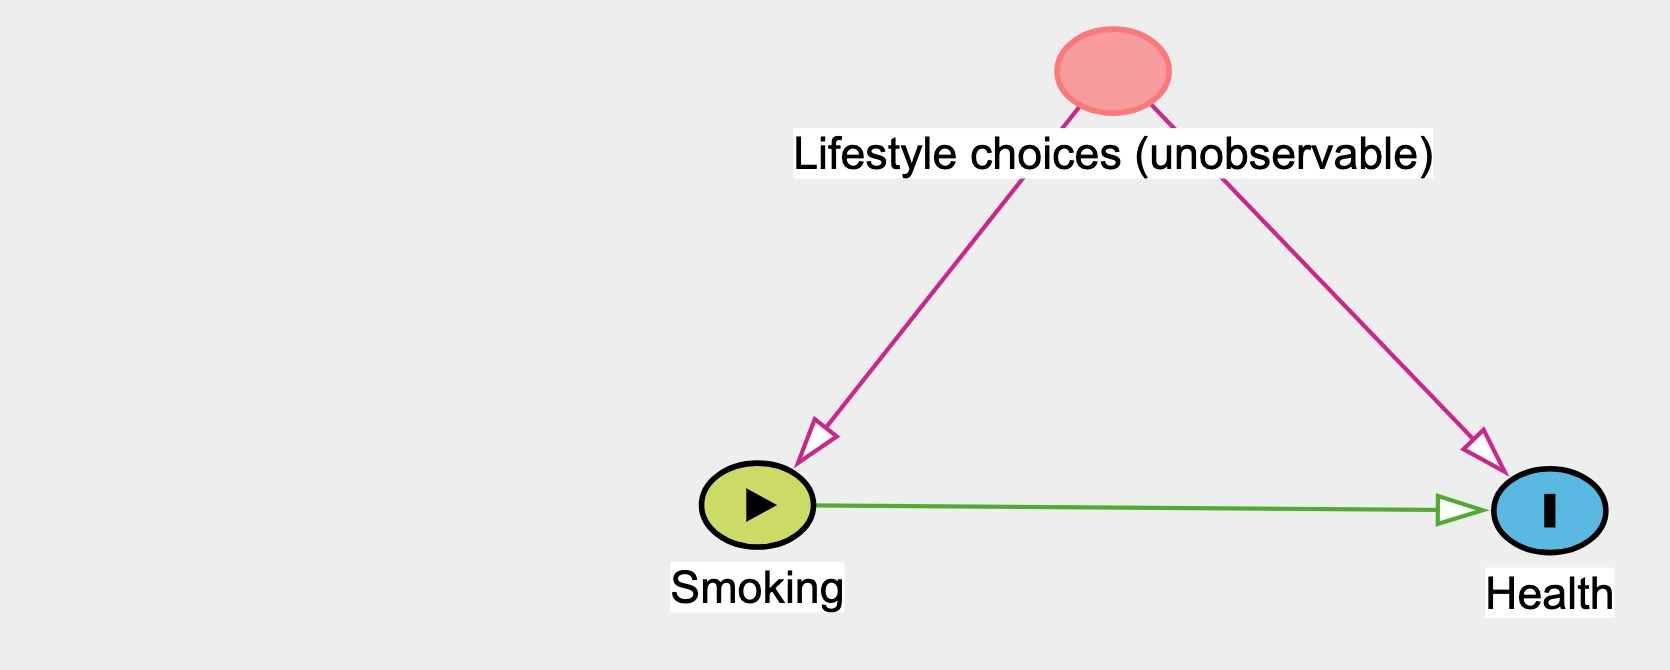
\includegraphics[width = 0.85\textwidth]{../img/smoking1}}

\end{frame}
% ----------------------------------------------------
\note{Quick recap of week 4. The diagram (Huntington-Klein, new to them) is the problem in one picture: lifestyle choices drive both smoking and health, and we will never measure them well enough to control them away.

So what do we do when the back door goes through something we cannot observe? That is today.}

% ----------------------------------------------------
\begin{frame}
\frametitle{The experimental fix}
\centering

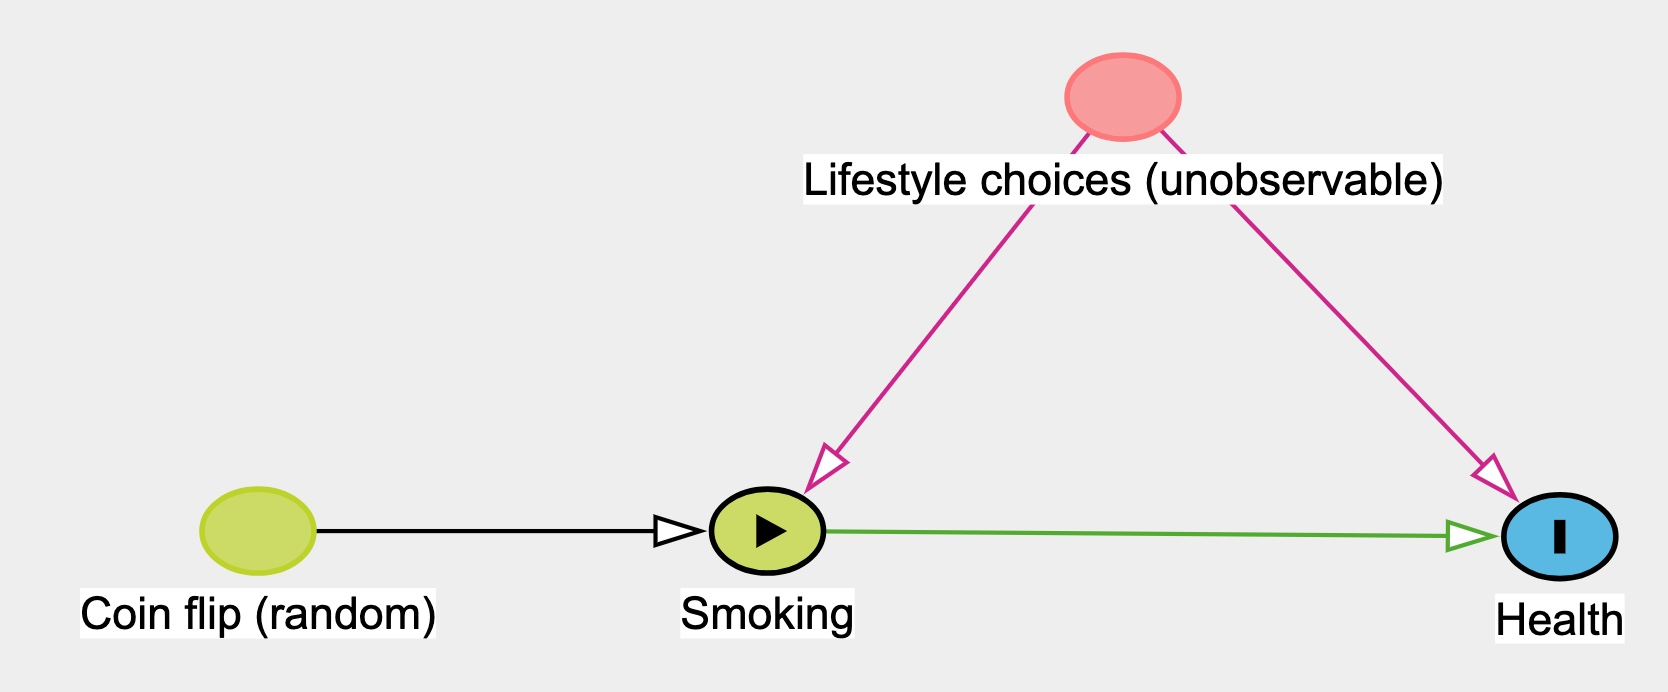
\includegraphics[width = 0.85\textwidth]{../img/smoking2}

\vspace{10pt}
{\small A coin flip moves smoking, and nothing else.\\ The back door is still there, but it no longer matters.}

\end{frame}
% ----------------------------------------------------
\note{This is what randomization does in DAG language. The coin creates variation in smoking that has nothing to do with lifestyle. If we only use \textbf{that} variation, the back door is irrelevant.

The whole of today follows from this picture. Every design template is a search for something that behaves like the coin flip, in data we did not design.}

% ====================================================
\section{Two strategies}
% ====================================================

% ----------------------------------------------------
\begin{frame}
\frametitle{Two ways of finding a stand-in}
\centering

\begin{itemize}
  \item[1.] \textbf{Close the back doors}
  \begin{itemize}
    \item controlling, matching, fixed effects
    \item works if you can name and measure (or hold constant) the confounders
  \end{itemize}
  \vspace{12pt}
  \item<2->[2.] \textbf{Find variation where they are closed by design}
  \begin{itemize}
    \item difference-in-differences, regression discontinuity, instrumental variables
    \item something moves the treatment for reasons unrelated to the outcome
  \end{itemize}
  \vspace{12pt}
  \item<3-> In practice, most good papers do both
\end{itemize}

\end{frame}
% ----------------------------------------------------
\note{The organising distinction for the first half. The first family works on the confounders; the second works on the source of variation in the treatment.

Huntington-Klein calls the second family ``template causal diagrams'': causal structures that show up often enough that we have names and standard checks for them. They are not magic estimators. They are recognisable situations.}

% ----------------------------------------------------
\begin{frame}
\frametitle{Back to Gary: who is his stand-in?}
\centering

\vspace{10pt}
\begin{itemize}
  \item<1-> A non-smoking neighbour of the same age, income, diet\ldots
  \begin{itemize}
    \item<1-> \textbf{controlling, matching}
  \end{itemize}
  \vspace{8pt}
  \item<2-> Gary compared with himself, or with his own family
  \begin{itemize}
    \item<2-> \textbf{fixed effects}
  \end{itemize}
  \vspace{8pt}
  \item<3-> Gary before he started, plus how non-smokers changed meanwhile
  \begin{itemize}
    \item<3-> \textbf{difference-in-differences}
  \end{itemize}
  \vspace{8pt}
  \item<4-> A Gary just old enough to buy cigarettes, or nudged into smoking by chance
  \begin{itemize}
    \item<4-> \textbf{regression discontinuity, instrumental variables}
  \end{itemize}
\end{itemize}

\end{frame}
% ----------------------------------------------------
\note{Delivering the promise from last week: each design is a different choice of stand-in for Gary, and each fails in its own way.
\begin{itemize}
  \item The neighbour differs in things we did not measure
  \item Gary-before is younger; the brother chose not to smoke for some reason
  \item The trend of non-smokers may not be Gary's trend
  \item The Gary at the age cutoff, or the one nudged by chance, may not be typical
\end{itemize}
Come back to this list at the summary table.}

% ----------------------------------------------------
\begin{frame}
\frametitle{Three questions for every design}
\centering

\vspace{15pt}
\begin{enumerate}
  \item[1.] What \textbf{variation} does it use?
  \vspace{15pt}
  \item[2.] What has to be \textbf{true} for that variation to be as good as random?
  \vspace{15pt}
  \item[3.] How could you \textbf{check}, at least partly?
\end{enumerate}

\vspace{20pt}
{\small \asher{No estimation today. That is for the causal inference course.}}

\end{frame}
% ----------------------------------------------------
\note{This is the template for the whole first half, and it is what I expect to hear in the workshop presentations.

Stress question 2. Every design rests on an assumption that cannot be fully tested. The difference between a good and a bad design is not whether it has such an assumption, but whether the assumption is plausible and whether you said it out loud.

Scope reminder: they will see estimators, standard errors and software elsewhere in the programme. Here we only care about the logic.}

% ====================================================
\section{Controlling and matching}
% ====================================================

% ----------------------------------------------------
\begin{frame}
\frametitle{Controlling, again}
\centering

\begin{itemize}
  \item When you control for $Z$, you compare units with the \textbf{same value of $Z$}
  \vspace{8pt}
  \item Subsetting is controlling too
  \begin{itemize}
    \item studying education $\rightarrow$ income only among people raised in big cities holds urban/rural constant
  \end{itemize}
  \vspace{8pt}
  \item<2-> \textbf{Matching} pushes this idea further
  \begin{itemize}
    \item for each treated unit, find untreated units that look the same on $Z$
    \item compare only within those matched pairs
  \end{itemize}
\end{itemize}

\end{frame}
% ----------------------------------------------------
\note{The intuition to transmit: regression with controls and matching do the same conceptual job. Both build the comparison among units that are alike on observed characteristics.

Nick Huntington-Klein's animations are good for this if there is time to show one: \url{https://www.nickchk.com/anim/Animation\%20of\%20Matching.gif}.}

% ----------------------------------------------------
\begin{frame}
\frametitle{Two ways to match}
\centering

\begin{itemize}
  \item \textbf{Distance matching}: pair units with similar values on each $Z$
  \vspace{8pt}
  \item \textbf{Propensity score}: estimate the probability of being treated given $Z$, then match on that one number
  \vspace{8pt}
  \item Usually you match controls to treated units $\rightarrow$ the \textbf{ATT}
  \vspace{8pt}
  \item<2-> Treated units with no comparable control are \textbf{dropped}
  \begin{itemize}
    \item<2-> the estimate is now about a different population
  \end{itemize}
\end{itemize}

\end{frame}
% ----------------------------------------------------
\note{Keep this light. The point to stress is \textbf{common support}: you can only compare treated units with controls that had a similar chance of being treated. Units with no comparable counterpart get dropped, and that changes the population the estimate is about.

Link to week 4: matching controls to treated units gives the effect on the treated (ATT), which is often the policy-relevant quantity anyway.}

% ----------------------------------------------------
\begin{frame}
\frametitle{What matching cannot do}
\centering

\vspace{10pt}
\begin{itemize}[<+->]
  \item Matching is \textbf{selection on observables}, just like regression
  \vspace{8pt}
  \item If lifestyle is unobserved, two matched ``identical'' people still differ in lifestyle
  \vspace{8pt}
  \item Matching makes the comparison look clean.\\ It does not make the confounder go away
\end{itemize}

\vspace{15pt}
\uncover<3->{{\small Variation used: treated vs.\ untreated, \textit{among units that look alike}\\Must be true: \textbf{no unobserved confounders}}}

\end{frame}
% ----------------------------------------------------
\note{The most common misunderstanding: matching is presented as more ``causal'' than regression because the tables look like an experiment. It isn't. The identifying assumption is identical: everything that matters is observed.

First use of the three questions. Ask them how they would check the assumption. Honest answer: you mostly cannot, which is why the rest of the templates exist. Sensitivity analysis (how strong would an unobserved confounder have to be?) is the partial check.}

% ====================================================
\section{Fixed effects}
% ====================================================

% ----------------------------------------------------
\begin{frame}
\frametitle{Fixed effects: compare within groups}
\centering

\begin{itemize}
  \item Some unobserved confounders are \textbf{constant within a group}
  \begin{itemize}
    \item country history, in a cross-national panel
    \item school, in a study of students
    \item the person, in a panel survey
    \item the user, in repeated platform data
  \end{itemize}
  \vspace{8pt}
  \item<2-> Then compare only \textbf{within} each group
  \begin{itemize}
    \item every group-level confounder is held constant, \textit{observed or not}
  \end{itemize}
\end{itemize}

\end{frame}
% ----------------------------------------------------
\note{Fixed effects are the first tool that handles unobservables, but only of one kind: those that do not vary within the group.

The user example is the one for this cohort. With repeated observations of the same account, everything stable about that person (personality, ideology, baseline activity) drops out when you compare the account to itself.}

% ----------------------------------------------------
\begin{frame}
\frametitle{Example: high school and university grades}
\centering

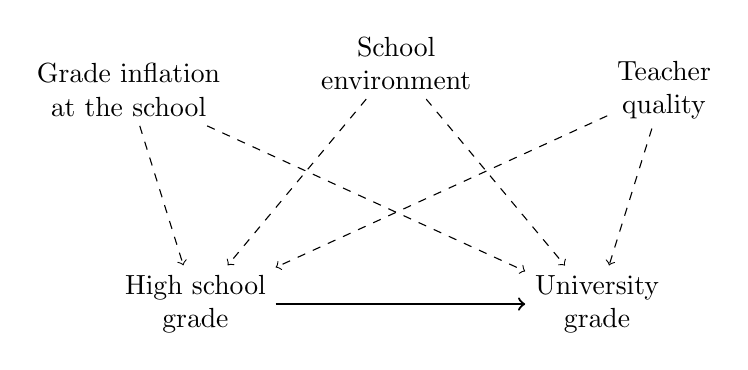
\begin{tikzpicture}[every text node part/.style={align=center}, scale = 0.85]
\node (D) at (-3,0){High school\\grade};
\node (Y) at (3,0){University\\grade};
\node (U1) at (-4,3.2){Grade inflation\\at the school};
\node (U2) at (0,3.6){School\\environment};
\node (U3) at (4,3.2){Teacher\\quality};
\draw[->, thick] (D) -- (Y);
\draw[->, dashed] (U1) -- (D);
\draw[->, dashed] (U1) -- (Y);
\draw[->, dashed] (U2) -- (D);
\draw[->, dashed] (U2) -- (Y);
\draw[->, dashed] (U3) -- (D);
\draw[->, dashed] (U3) -- (Y);
\end{tikzpicture}

\vspace{15pt}
{\small All the dashed arrows come from the \textbf{school}. We can't measure them, but we know which school each student went to}

\end{frame}
% ----------------------------------------------------
\note{Question: do high school grades predict university grades? Lots of confounders, none of them easy to measure. But they share one feature: they are properties of the school, and every student in a school shares them.

So instead of measuring them, we compare students only to classmates from the same school.}

% ----------------------------------------------------
\begin{frame}[plain]
  \begin{tikzpicture}[remember picture, overlay]
    \node[at = (current page.center), yshift = 0cm] (cover) {%
      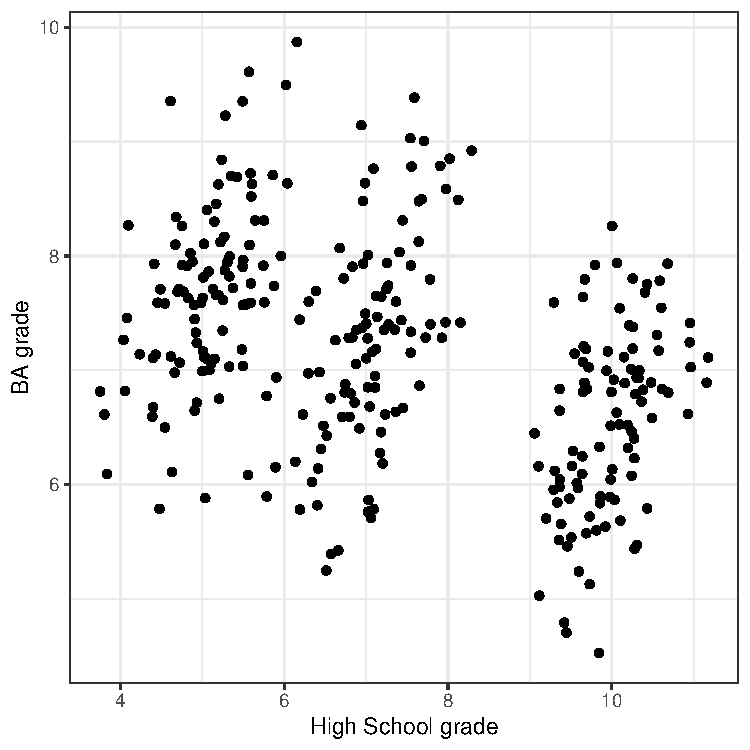
\includegraphics[keepaspectratio, height=.85\paperheight]{../img/fe1}};
  \end{tikzpicture}
\end{frame}
% ----------------------------------------------------
\note{Simulated data. Pooling all students, the relationship looks flat or even negative: students with the highest high school grades do worse at university.

Ask: what would you conclude from this plot? Then ask what might be hiding in it.}

% ----------------------------------------------------
\begin{frame}[plain]
  \begin{tikzpicture}[remember picture, overlay]
    \node[at = (current page.center), yshift = 0cm] (cover) {%
      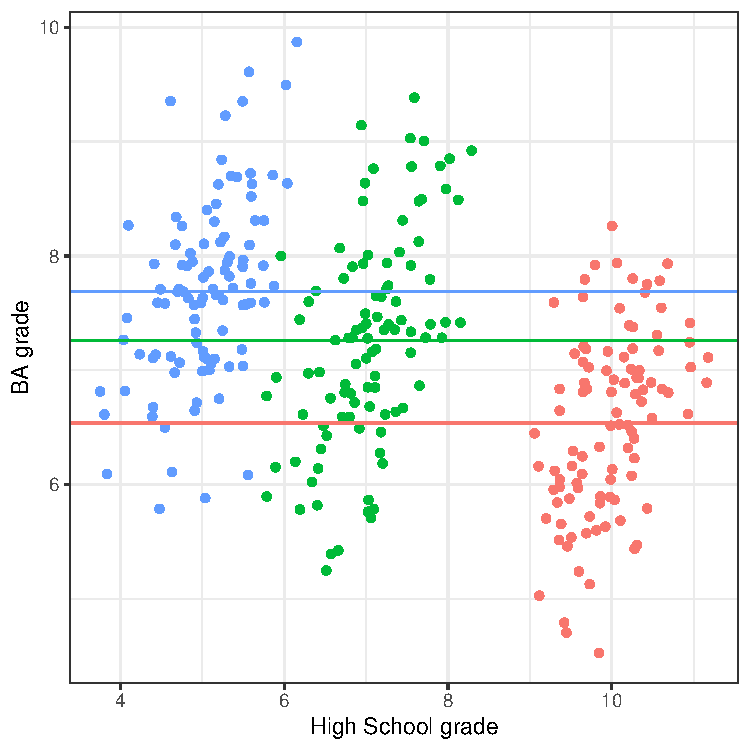
\includegraphics[keepaspectratio, height=.85\paperheight]{../img/fe5}};
  \end{tikzpicture}
\end{frame}
% ----------------------------------------------------
\note{Colour by school. Three schools, and the red one inflates grades: its students get high marks in high school and then do worse at university. The horizontal lines are the school means.

Within each school, the relationship is clearly positive. The pooled pattern was driven by differences between schools.}

% ----------------------------------------------------
\begin{frame}[plain]
  \begin{tikzpicture}[remember picture, overlay]
    \node[at = (current page.center), yshift = 0cm] (cover) {%
      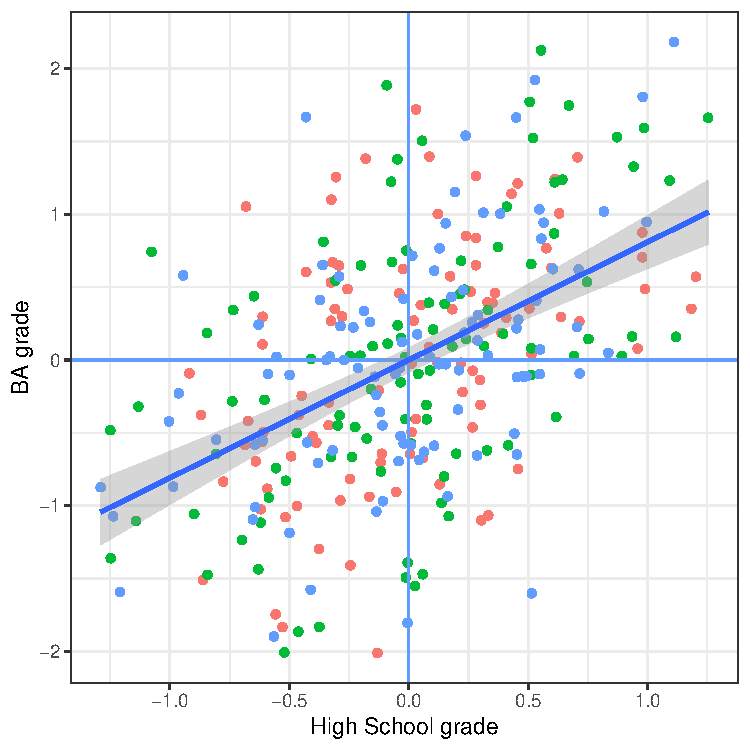
\includegraphics[keepaspectratio, height=.85\paperheight]{../img/fe9}};
  \end{tikzpicture}
\end{frame}
% ----------------------------------------------------
\note{This is what fixed effects do: subtract each school's mean from both variables, so every student is measured relative to their classmates. All between-school differences are gone, and the within-school slope appears.

Name it: this is Simpson's paradox, and fixed effects are the design answer to it. Also connects to the ecological fallacy from earlier sessions.}

% ----------------------------------------------------
\begin{frame}
\frametitle{What fixed effects cannot do}
\centering

\begin{itemize}[<+->]
  \item Confounders that \textbf{change within the group}
  \begin{itemize}
    \item a new head teacher, a policy change mid-panel
  \end{itemize}
  \vspace{8pt}
  \item Treatments that \textbf{do not vary within the group}
  \begin{itemize}
    \item all between-group variation is thrown away
  \end{itemize}
  \vspace{8pt}
  \item Reverse causality within the group
\end{itemize}

\vspace{15pt}
\uncover<3->{{\small Variation used: differences \textit{within} groups\\Must be true: \textbf{no confounders that vary within groups}}}

\end{frame}
% ----------------------------------------------------
\note{Three questions again. The assumption is weaker than selection on observables, but it is still an assumption.

The second point is a real cost that students underestimate: if most of the interesting variation is between countries, country fixed effects leave you with very little, and with the units whose treatment happened to change. Ask: who are those units, and are they typical?}

% ====================================================
\section{Difference-in-differences}
% ====================================================

% ----------------------------------------------------
\begin{frame}
\frametitle{Something changes at a moment in time}
\centering

\begin{itemize}
  \item A minimum wage increase, a terrorist attack, a platform changes its algorithm, a town renames its streets
  \vspace{8pt}
  \item<2-> Naive comparison 1: \textbf{before vs.\ after}, in treated units
  \begin{itemize}
    \item but other things changed over time too
  \end{itemize}
  \vspace{8pt}
  \item<3-> Naive comparison 2: \textbf{treated vs.\ untreated}, after
  \begin{itemize}
    \item but they were different to begin with
  \end{itemize}
  \vspace{8pt}
  \item<4-> \textbf{DiD}: use the untreated group's change over time as the counterfactual for the treated
\end{itemize}

\end{frame}
% ----------------------------------------------------
\note{Concrete example from my own work: Spanish municipalities that removed Francoist street names. Did removal change support for Vox?
\begin{itemize}
  \item Before/after in removing towns: Vox grew everywhere between 2015 and 2019, so the change mixes the treatment with a national trend
  \item Removers vs.\ non-removers after: removers were more left-wing to begin with
\end{itemize}
DiD combines both comparisons, and each one fixes the other's problem.}

% ----------------------------------------------------
\begin{frame}[plain]
  \begin{tikzpicture}[remember picture, overlay]
    \node[at = (current page.center), yshift = 0cm] (cover) {%
      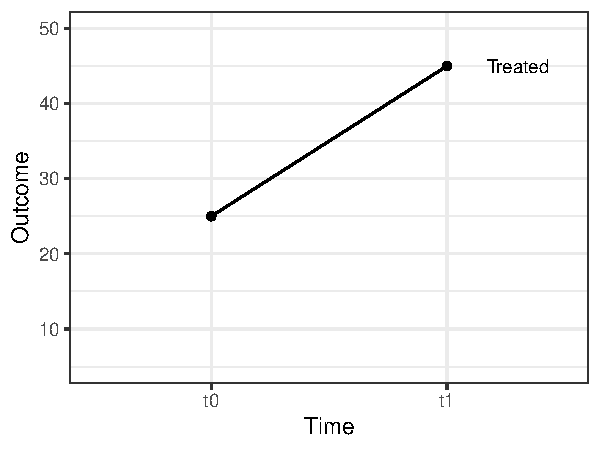
\includegraphics[keepaspectratio, width=.9\paperwidth]{../img/did1}};
  \end{tikzpicture}
\end{frame}
% ----------------------------------------------------
\note{The treated group goes from 25 to 45. Is the effect 20? Only if nothing else would have changed.}

% ----------------------------------------------------
\begin{frame}[plain]
  \begin{tikzpicture}[remember picture, overlay]
    \node[at = (current page.center), yshift = 0cm] (cover) {%
      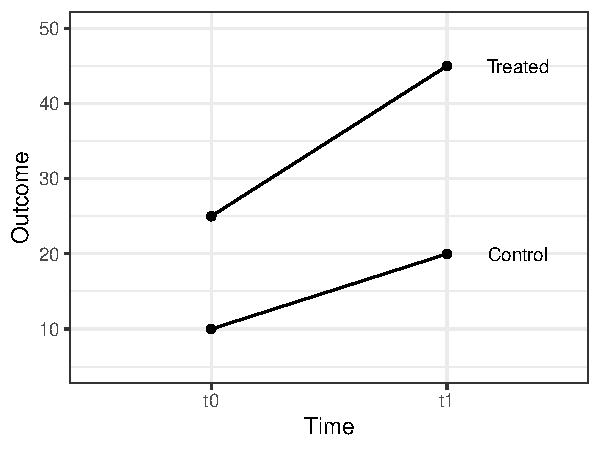
\includegraphics[keepaspectratio, width=.9\paperwidth]{../img/did2}};
  \end{tikzpicture}
\end{frame}
% ----------------------------------------------------
\note{Add a control group. It starts lower (they are different units) and rises by 10 over the same period, without treatment.}

% ----------------------------------------------------
\begin{frame}[plain]
  \begin{tikzpicture}[remember picture, overlay]
    \node[at = (current page.center), yshift = 0cm] (cover) {%
      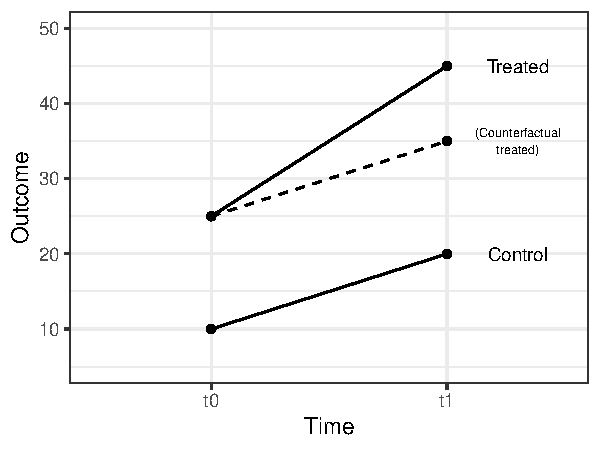
\includegraphics[keepaspectratio, width=.9\paperwidth]{../img/did3}};
  \end{tikzpicture}
\end{frame}
% ----------------------------------------------------
\note{The dashed line is the counterfactual: where the treated group would have been without treatment, assuming it would have followed the control group's trend.

This is the stand-in for Gary. Not the control group's level, but its \textbf{change}.}

% ----------------------------------------------------
\begin{frame}[plain]
  \begin{tikzpicture}[remember picture, overlay]
    \node[at = (current page.center), yshift = 0cm] (cover) {%
      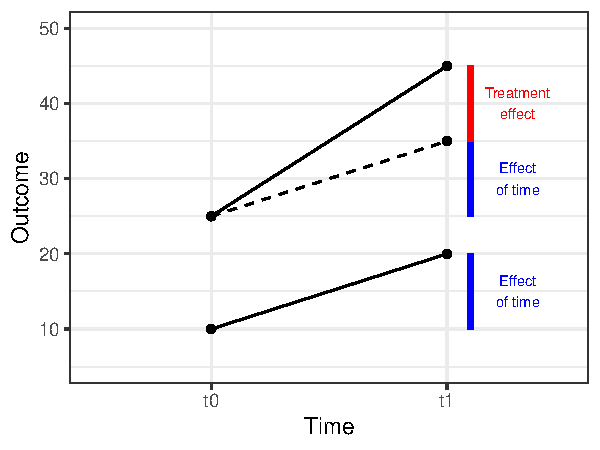
\includegraphics[keepaspectratio, width=.9\paperwidth]{../img/did5}};
  \end{tikzpicture}
\end{frame}
% ----------------------------------------------------
\note{Treated change (20) minus control change (10) = 10. Two differences, hence the name.

What it removes: anything constant about the groups (level differences) and anything that changes over time for everyone (common shocks). What it does not remove: anything that changes over time \textbf{differently} for the two groups.}

% ----------------------------------------------------
\begin{frame}
\frametitle{The first DiD? Cholera in London, 1850s}
\centering

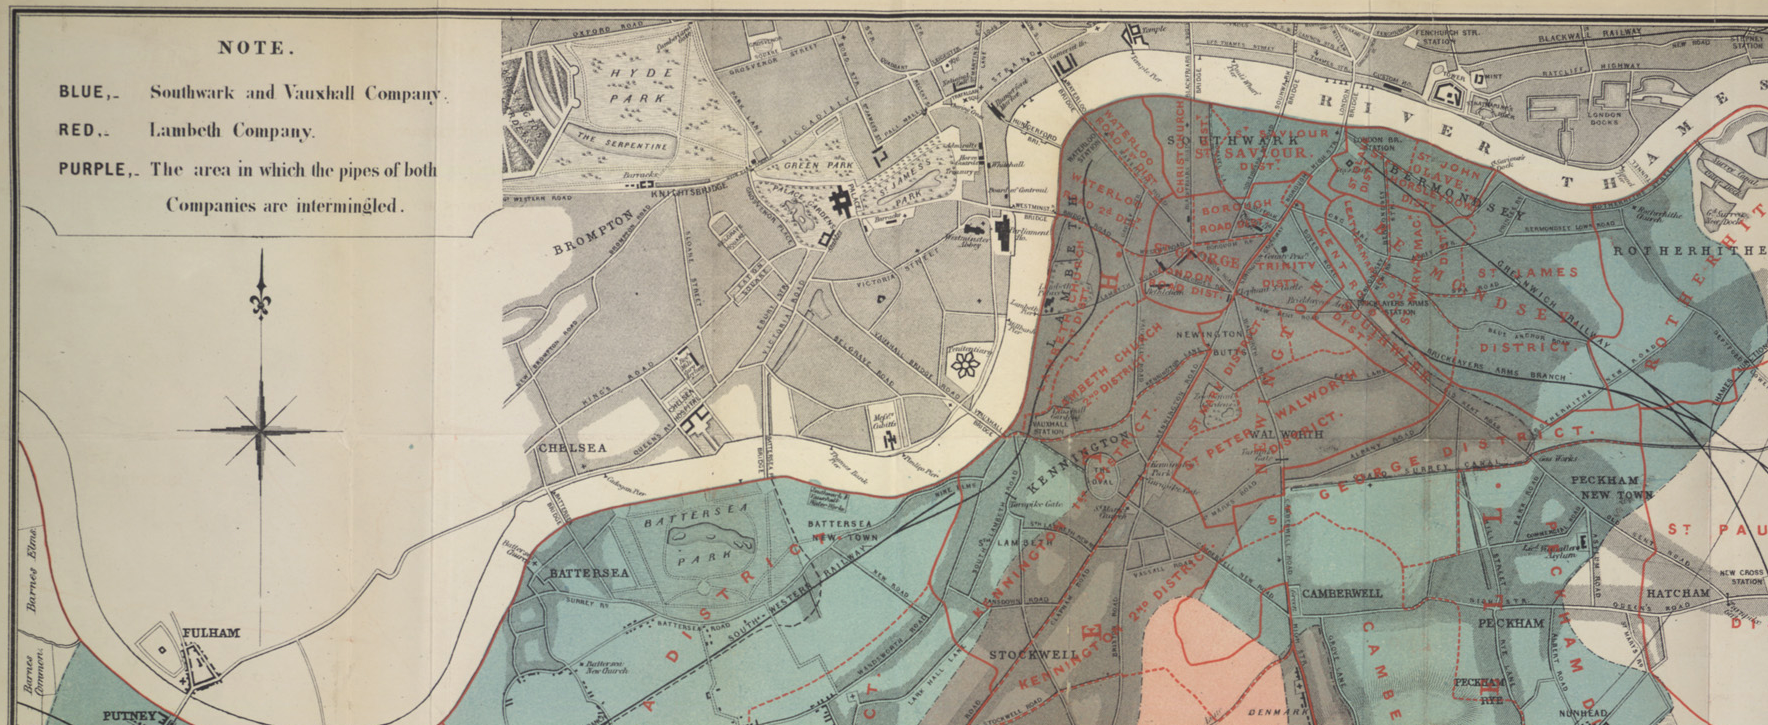
\includegraphics[width = \textwidth]{../img/snow_map}

\vspace{8pt}
\begin{itemize}
  \item The Lambeth company moved its water intake upriver in 1852. Southwark \& Vauxhall did not
  \item John Snow compared cholera deaths in their customers' homes before and after
\end{itemize}

\end{frame}
% ----------------------------------------------------
\note{The classic natural experiment. Both companies supplied the same neighbourhoods, often alternating houses on the same street, so customers were very similar.

Deaths fell sharply among Lambeth customers between the 1849 and 1854 outbreaks, and rose among Southwark \& Vauxhall customers. Snow did not have a regression; he had a table of four numbers. Good design does most of the work.}

% ----------------------------------------------------
\begin{frame}
\frametitle{The key assumption: parallel trends}
\centering

\begin{itemize}
  \item Without treatment, both groups would have \textbf{changed in the same way}
  \vspace{8pt}
  \item Not testable after treatment (that's the counterfactual). But partly checkable:
  \begin{itemize}
    \item<2-> look at \textbf{pre-treatment trends}: were they parallel before?
    \item<3-> ask \textbf{why} these units were treated now
  \end{itemize}
  \vspace{8pt}
  \item<4-> Threats: anticipation, other changes at the same time, selection into treatment based on trends, \textbf{spillovers} to the control group
\end{itemize}

\vspace{10pt}
\uncover<4->{{\small Variation used: changes over time, treated vs.\ untreated\\Must be true: \textbf{parallel trends}}}

\end{frame}
% ----------------------------------------------------
\note{Pre-trends are the standard check, and they need data from several periods before treatment. Parallel before does not guarantee parallel after, but diverging before is a strong warning.

The ``why now'' question is the important one for design. Towns that removed Francoist streets did so after a change of local government, and that change could itself affect voting. Policies are often adopted in response to trends in the outcome (Ashenfelter's dip: people enrol in training programmes after their earnings drop).}

% ----------------------------------------------------
\begin{frame}
\frametitle{When units are treated at different times}
\centering

\begin{minipage}{0.48\textwidth}
\begin{itemize}
  \item \textbf{Staggered} adoption is the normal case
  \vspace{8pt}
  \item Standard two-way fixed effects can then compare late-treated units with early-treated ones
  \vspace{8pt}
  \item If effects change over time, that comparison is biased
  \vspace{8pt}
  \item {\footnotesize See Goodman-Bacon (2021), Callaway \& Sant'Anna (2021), Roth et al.\ (2023)}
\end{itemize}
\end{minipage}\hfill
\begin{minipage}{0.48\textwidth}\centering
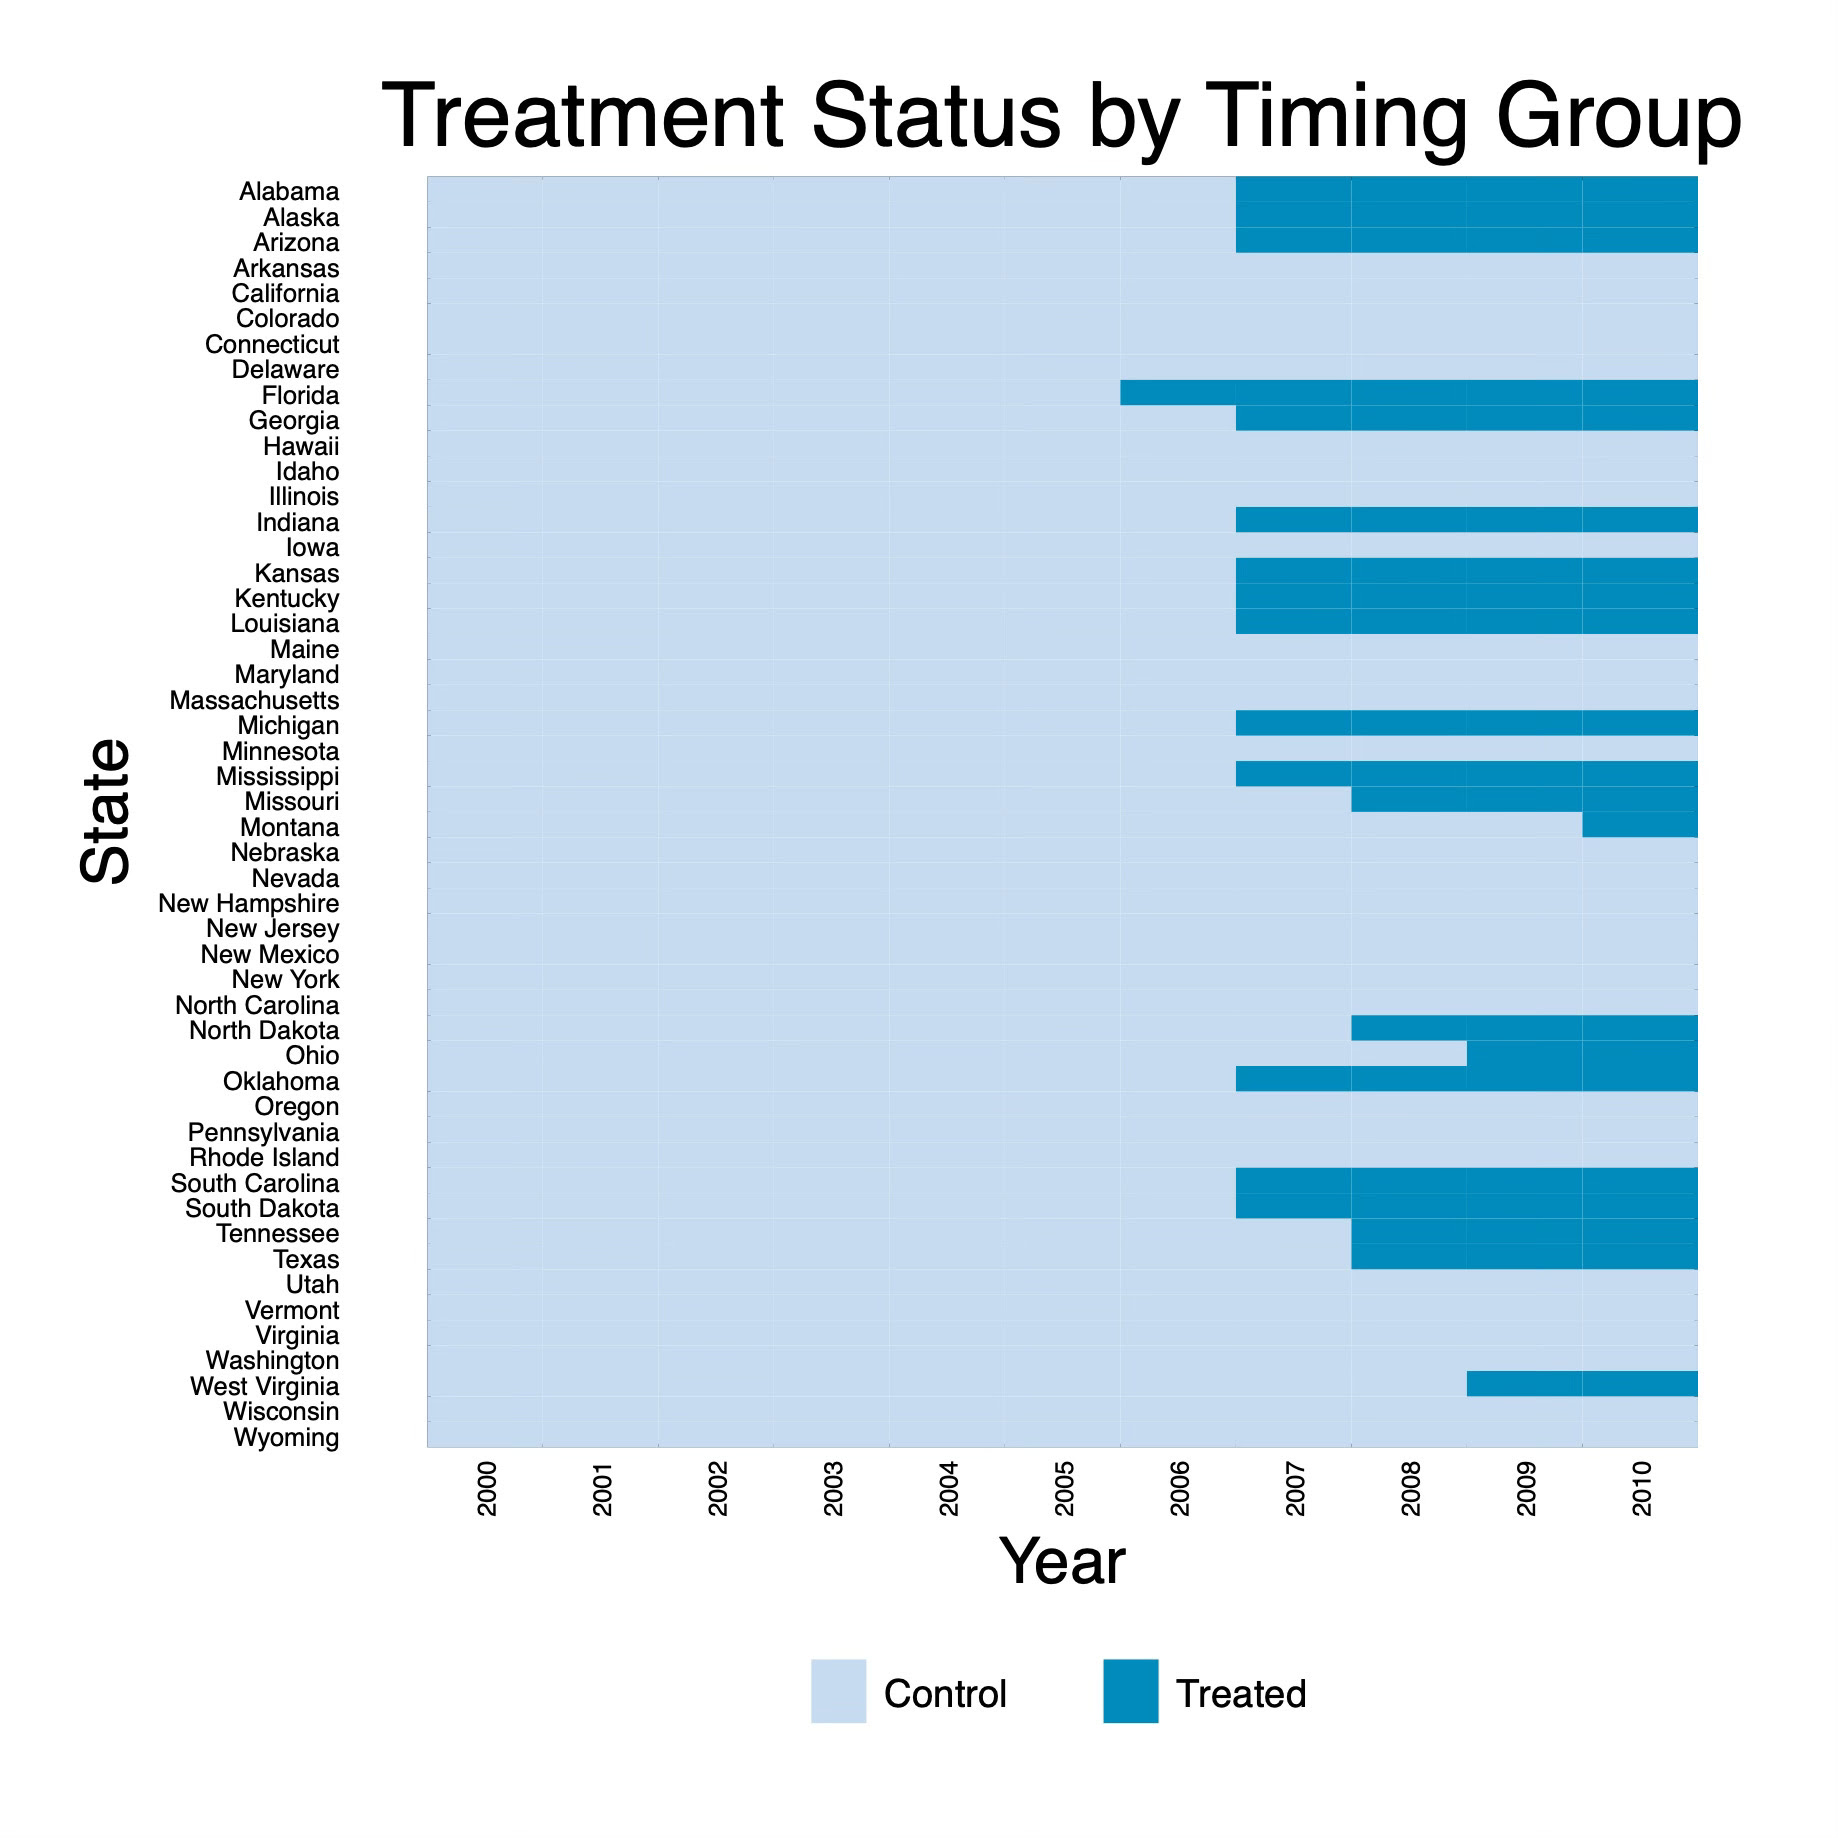
\includegraphics[width = \textwidth]{../img/staggered1}
\end{minipage}

\end{frame}
% ----------------------------------------------------
\note{(Optional, skip if short of time.) One slide only, as a flag. The figure shows US states adopting a policy in different years.

For design purposes the lesson is simple: know who your comparison group is at each moment. Already-treated units are not a valid control if the effect is still unfolding. The new estimators fix this by comparing each cohort only with not-yet-treated or never-treated units. They will see the details elsewhere.}

% ====================================================
\section{Regression discontinuity}
% ====================================================

% ----------------------------------------------------
\begin{frame}
\frametitle{Treatment assigned by a cutoff}
\centering

\begin{itemize}
  \item Treatment switches on when a \textbf{running variable} crosses a threshold
  \begin{itemize}
    \item winning an election (vote share above 50\%)
    \item a scholarship (test score above $x$)
    \item living on one side of a border (distance)
    \item being old enough to vote or be drafted (birth date)
  \end{itemize}
  \vspace{8pt}
  \item<2-> Far from the cutoff, units differ in many ways
  \item<2-> \textbf{Right at the cutoff}, they should be almost identical
\end{itemize}

\end{frame}
% ----------------------------------------------------
\note{The intuition: a candidate who wins with 50.1\% and one who loses with 49.9\% are basically the same kind of candidate in the same kind of district. Which side of 50\% they fell on is close to a coin flip.

That is the local randomisation idea. Ask them for examples of cutoffs in their own fields; there are a lot more than they think (eligibility thresholds, platform follower counts that unlock features, age limits).}

% ----------------------------------------------------
\begin{frame}[plain]
  \begin{tikzpicture}[remember picture, overlay]
    \node[at = (current page.center), yshift = 0cm] (cover) {%
      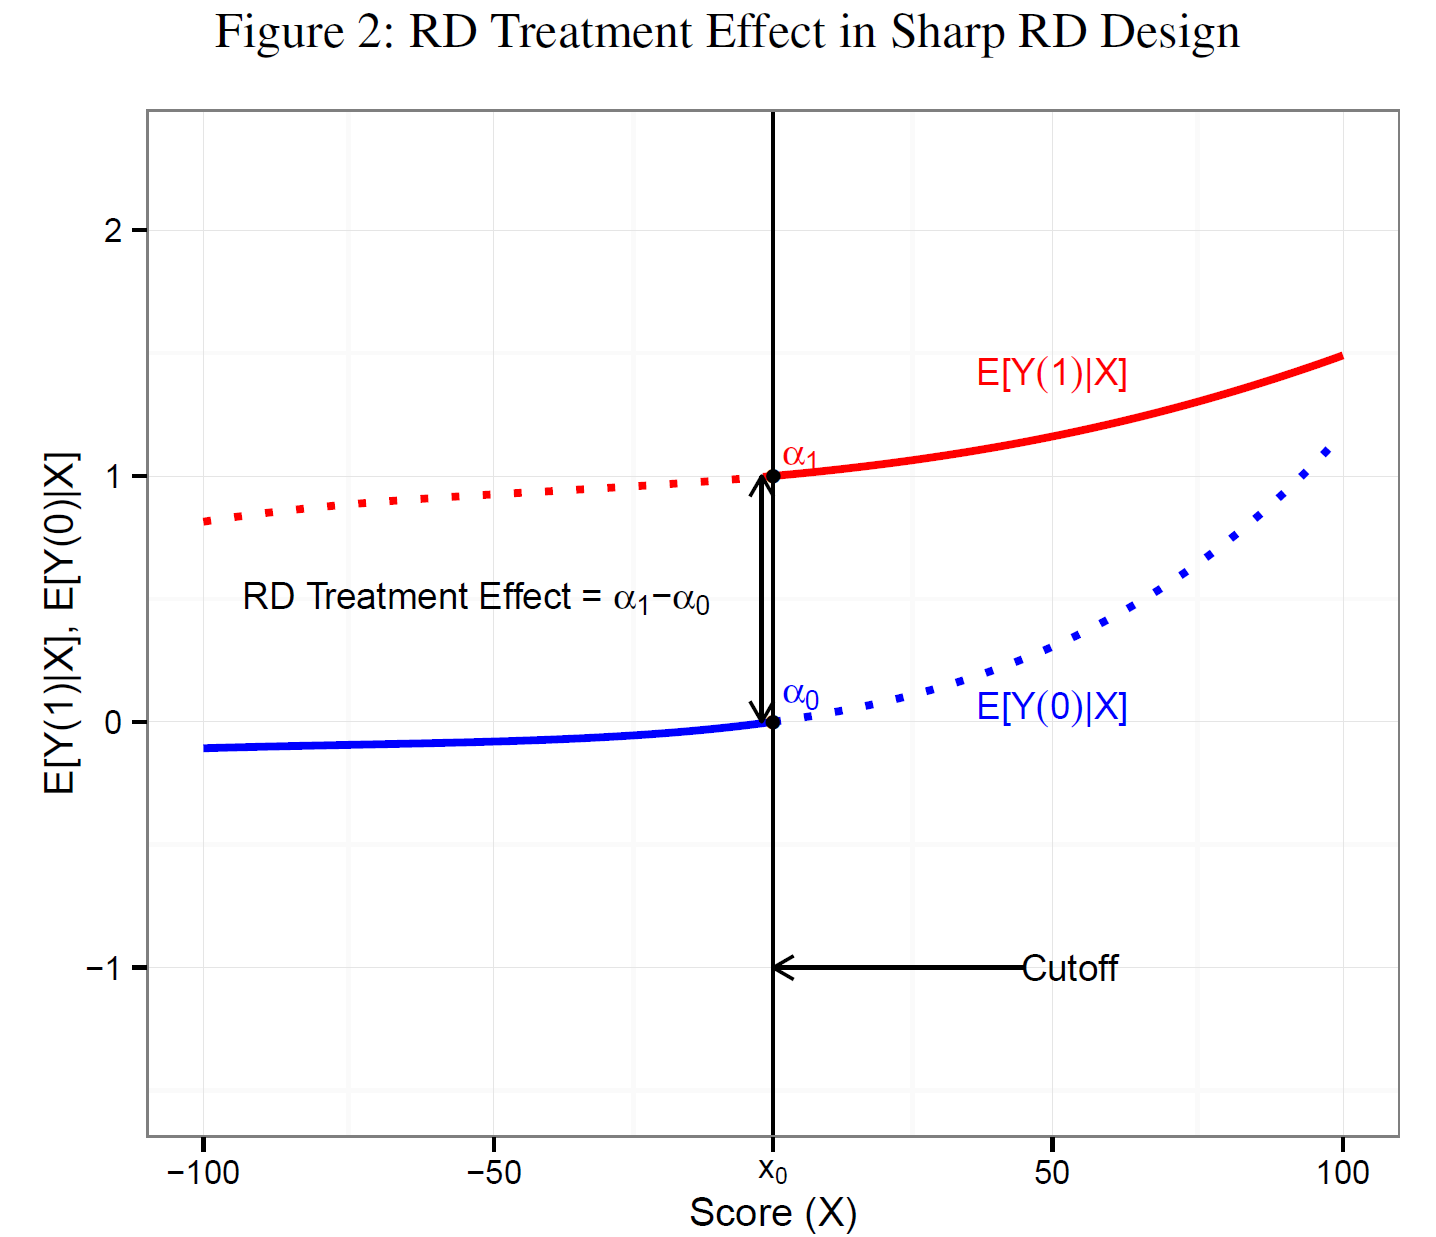
\includegraphics[keepaspectratio, height=.85\paperheight]{../img/rdd_teffect}};
  \end{tikzpicture}
\end{frame}
% ----------------------------------------------------
\note{The outcome changes smoothly with the running variable on both sides, and jumps at the cutoff. The jump is the effect.

Note the general slope: the running variable is clearly related to the outcome, so a naive treated-vs-untreated comparison would be confounded. RDD only uses the jump.}

% ----------------------------------------------------
\begin{frame}
\frametitle{Example: emancipation and Jewish national identity}
\centering

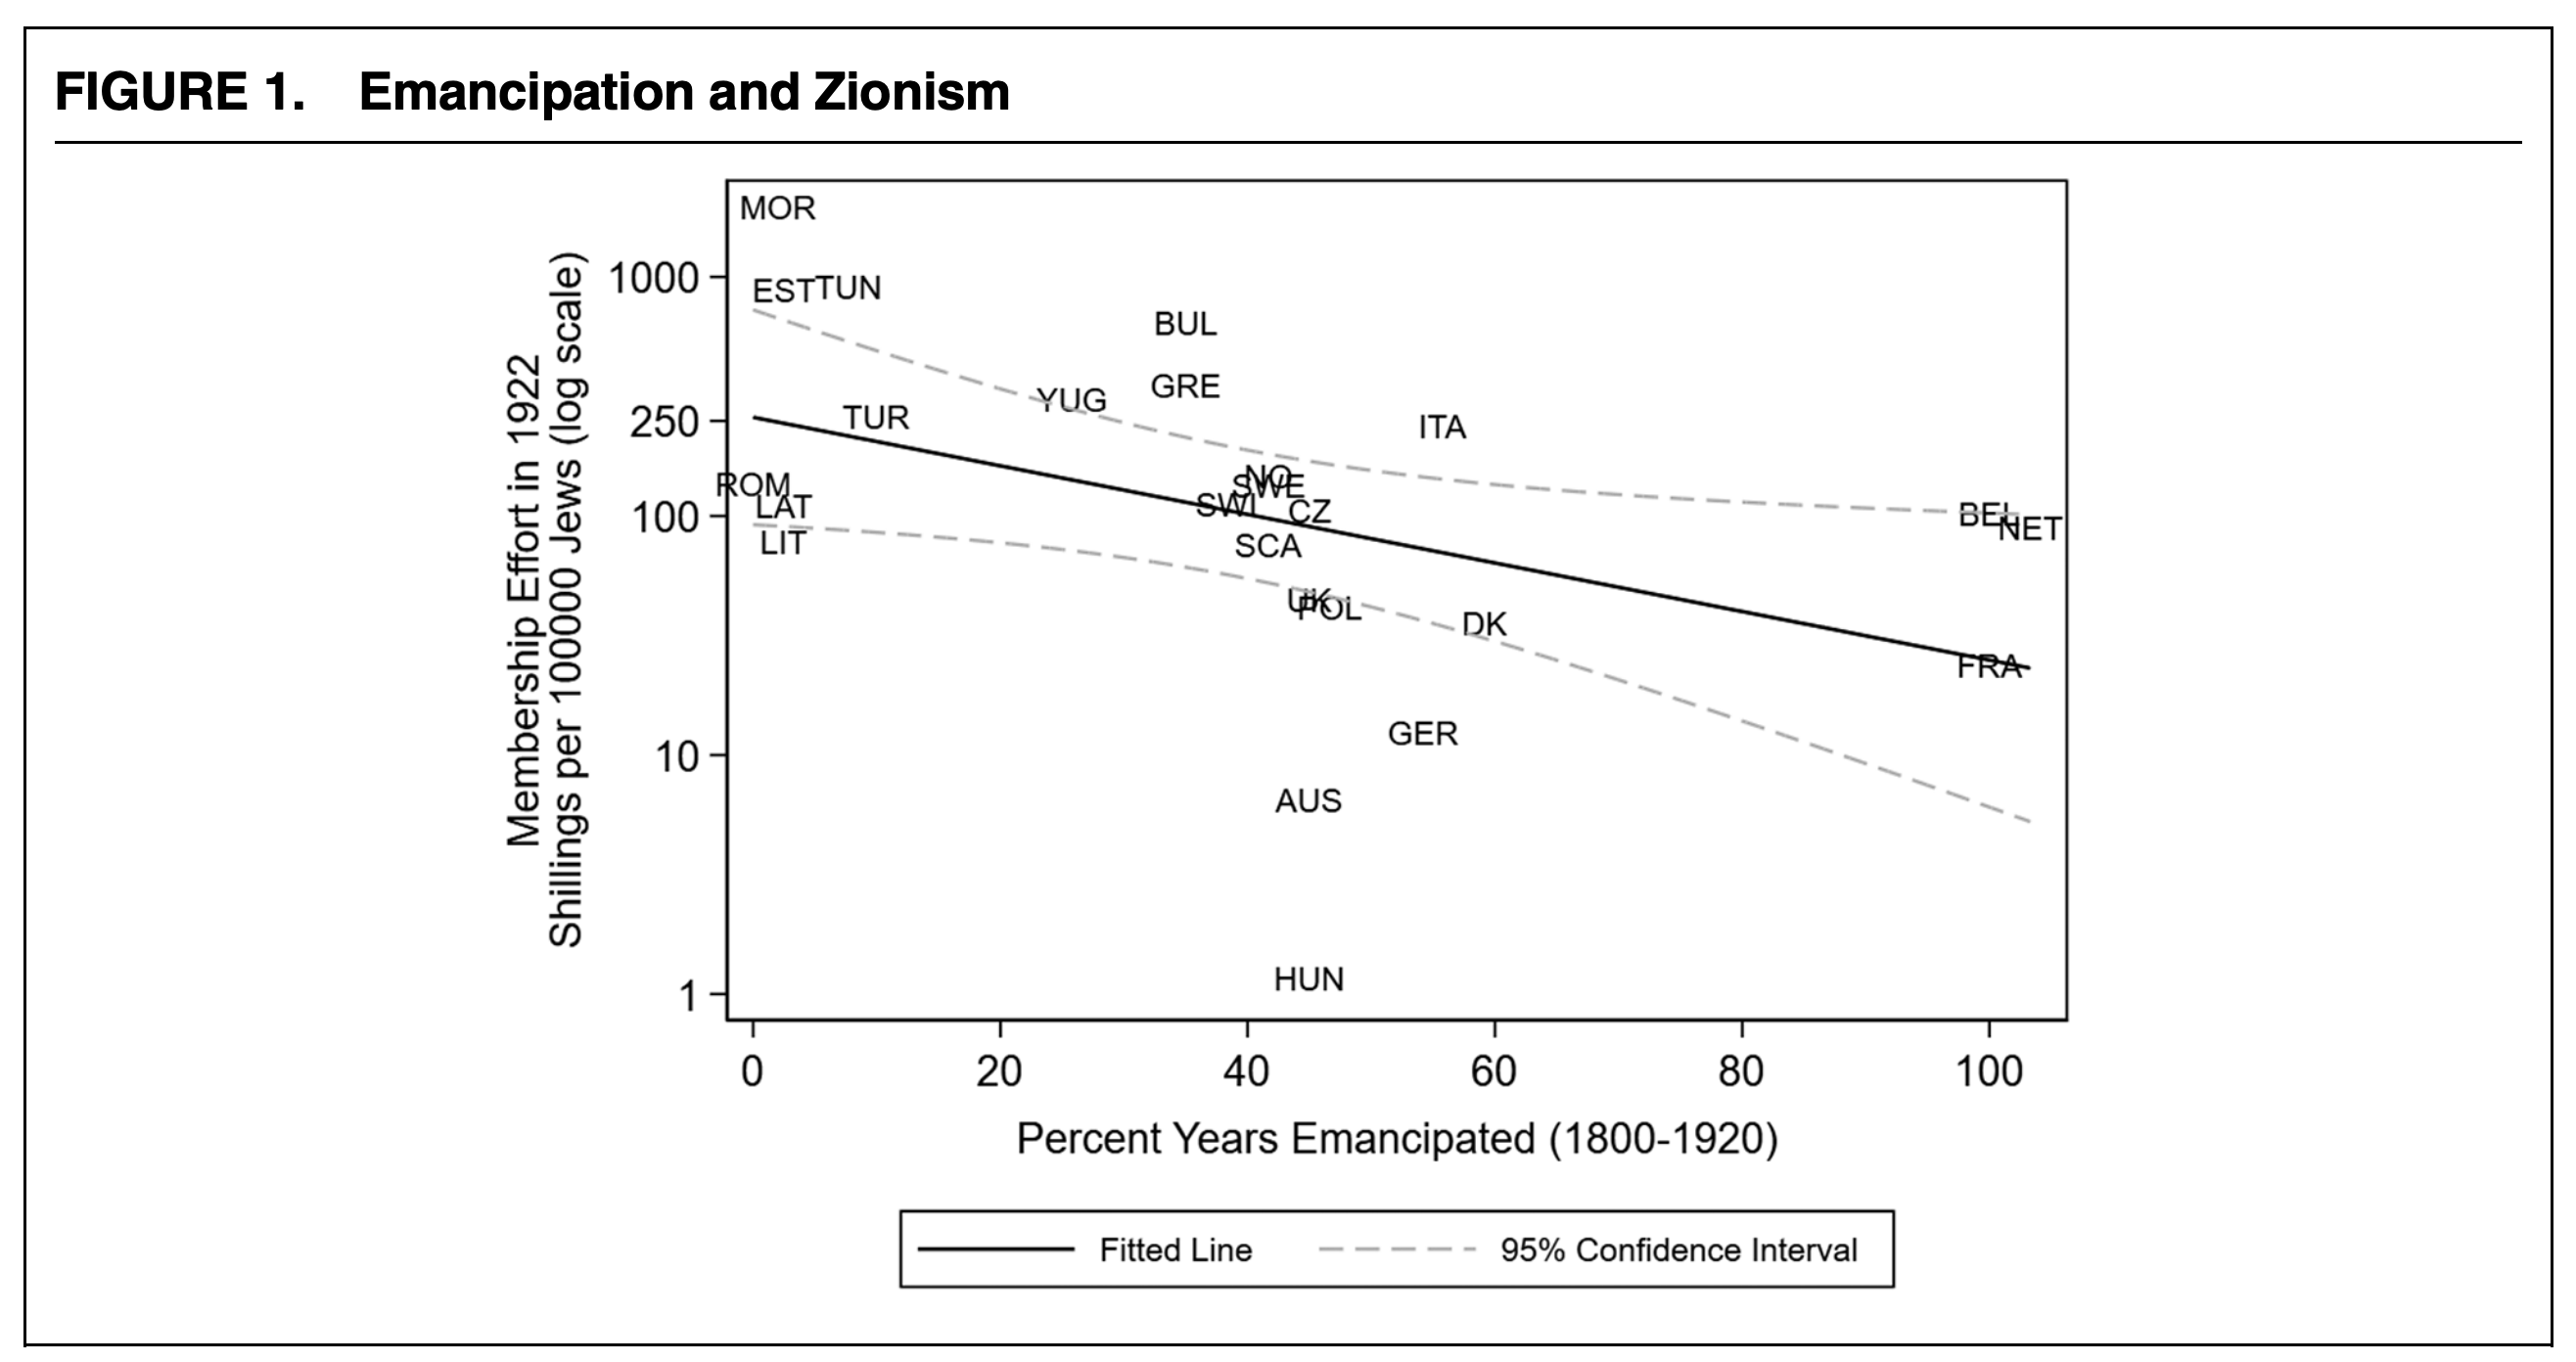
\includegraphics[width = 0.85\textwidth]{../img/boix_jewish2}

\vspace{5pt}
{\footnotesize Boix (2025), \textit{APSR}}

\end{frame}
% ----------------------------------------------------
\note{The question: did political emancipation shape whether Jews came to see themselves as a separate nation (Zionism)? Cross-nationally, the longer Jews had been emancipated, the weaker Zionist membership in 1922.

Ask: why is this plot not enough? Emancipated countries were richer, more urban, more liberal, and so on. Classic confounding across countries.}

% ----------------------------------------------------
\begin{frame}[plain]
  \begin{tikzpicture}[remember picture, overlay]
    \node[at = (current page.center), yshift = 0cm] (cover) {%
      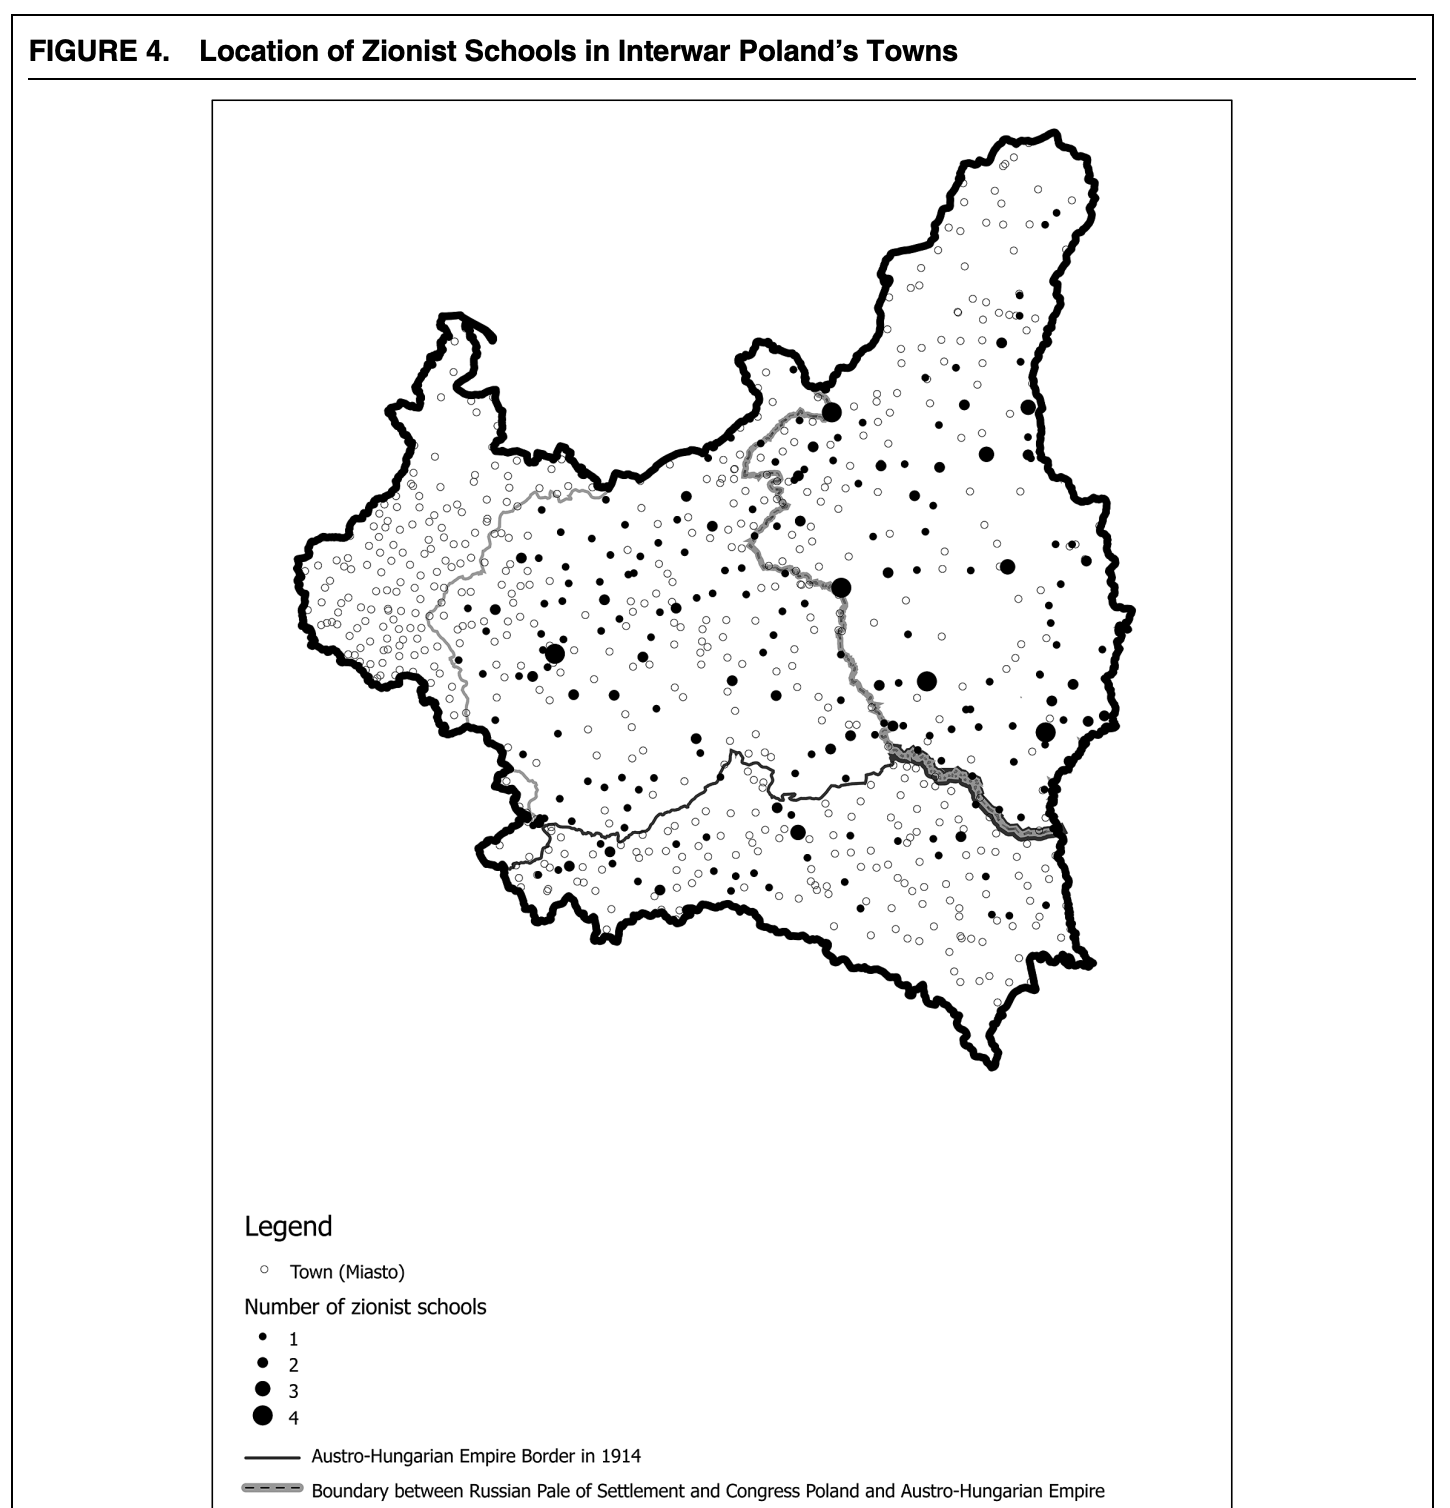
\includegraphics[keepaspectratio, height=.95\paperheight]{../img/boix_jewish3}};
  \end{tikzpicture}
\end{frame}
% ----------------------------------------------------
\note{The design: within interwar Poland, the old boundary between the Russian Pale of Settlement and Congress Poland. Jews on the two sides lived under different legal regimes under Tsarism, with the Pale far more restrictive. After 1918 they were in the same country.

The running variable is distance to the boundary. Towns just on either side should be similar in everything except their history of legal treatment.}

% ----------------------------------------------------
\begin{frame}[plain]
  \begin{tikzpicture}[remember picture, overlay]
    \node[at = (current page.center), yshift = 0cm] (cover) {%
      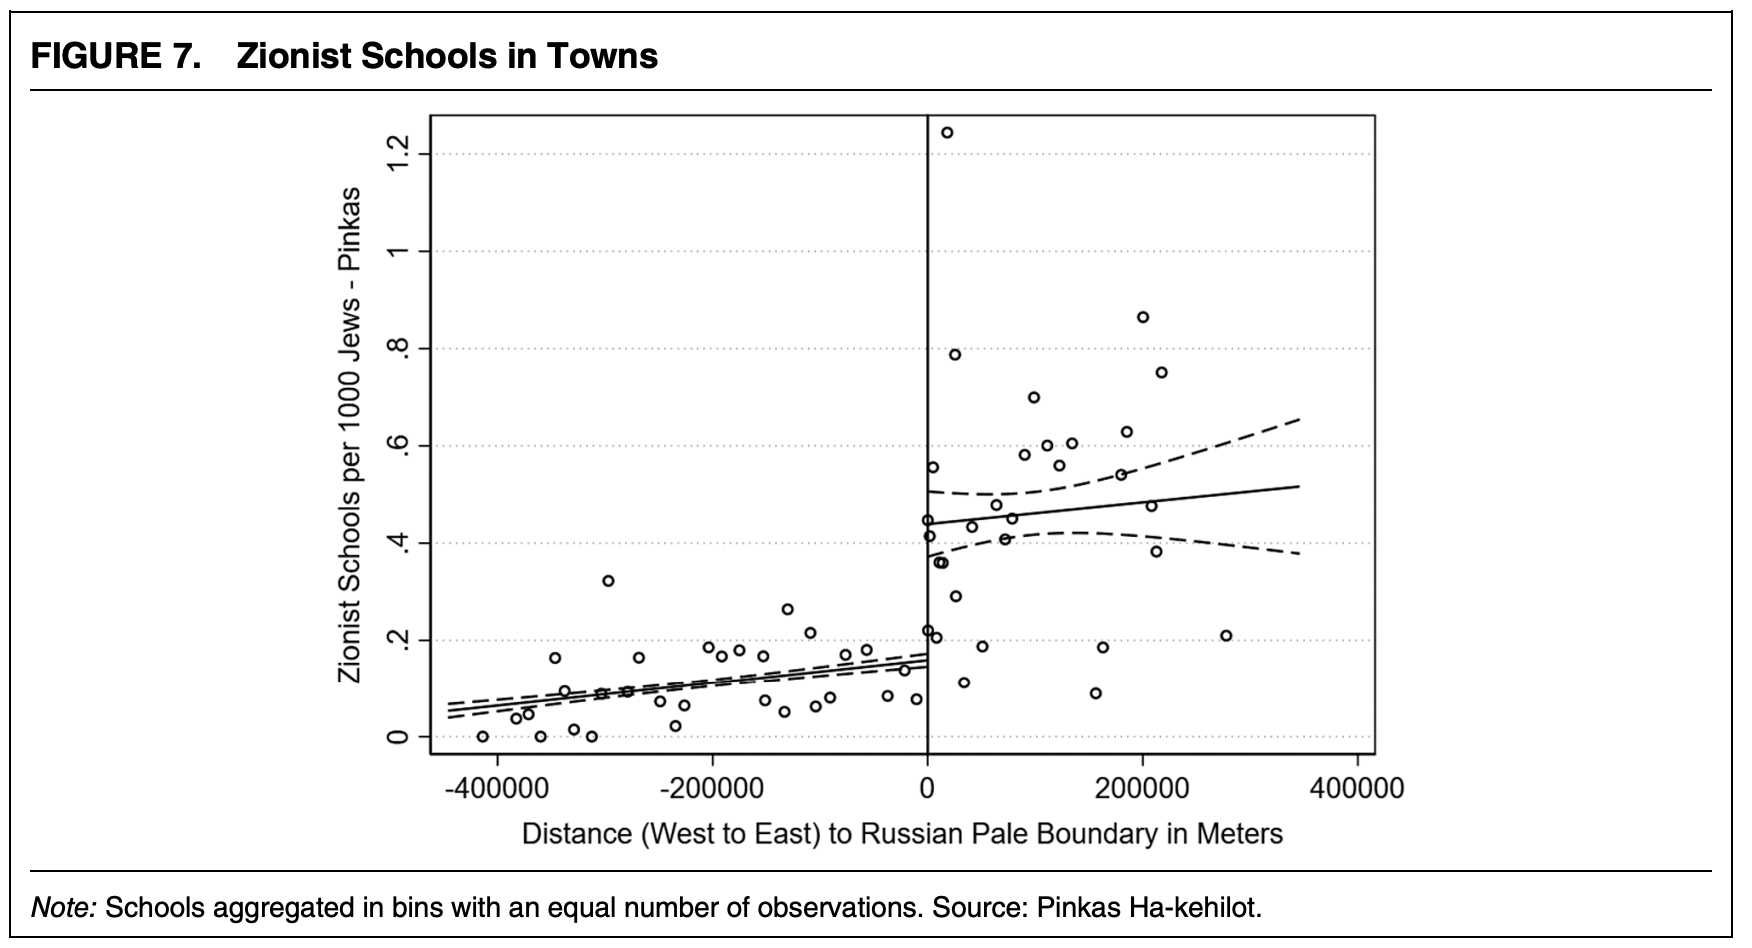
\includegraphics[keepaspectratio, width=.95\paperwidth]{../img/boix_jewish5}};
  \end{tikzpicture}
\end{frame}
% ----------------------------------------------------
\note{The jump: more Zionist schools per Jewish population just inside the Pale.

Ask: what would worry you? Pre-existing differences right at the border; the border coinciding with other things (language, religion, economic integration); people moving across it.}

% ----------------------------------------------------
\begin{frame}[plain]
  \begin{tikzpicture}[remember picture, overlay]
    \node[at = (current page.center), yshift = 0cm] (cover) {%
      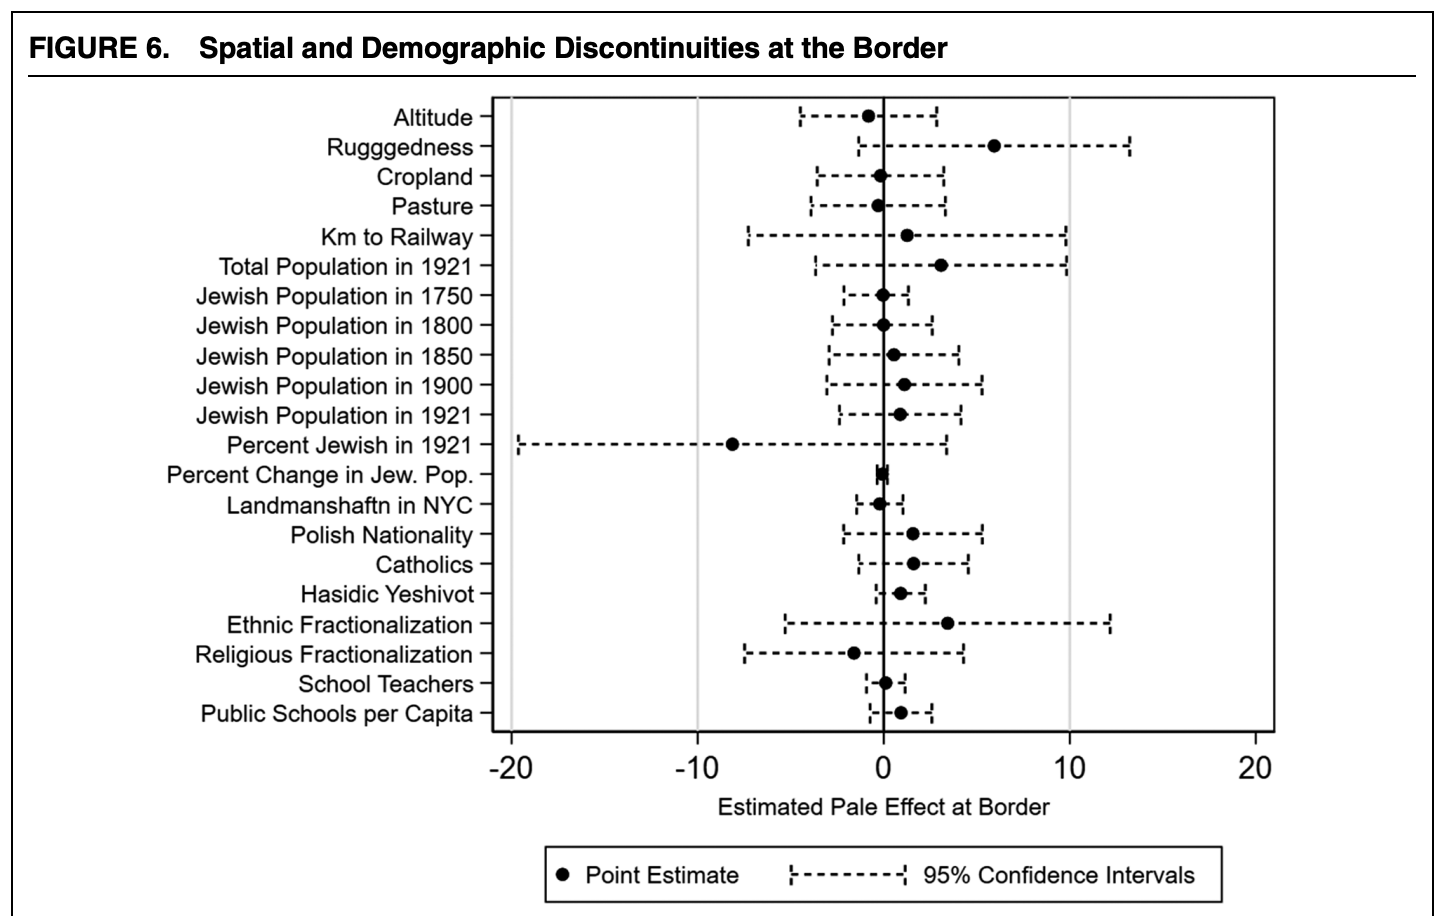
\includegraphics[keepaspectratio, width=.95\paperwidth]{../img/boix_jewish4}};
  \end{tikzpicture}
\end{frame}
% ----------------------------------------------------
\note{The check: run the same RDD on things that should \textbf{not} jump at the border. Geography, historical Jewish population, religion, schools. None of them do.

This is a balance test, and it is also a placebo test (more on these later). It is the closest RDD gets to showing that the cutoff behaves like a coin flip.}

% ----------------------------------------------------
\begin{frame}
\frametitle{Threats: what if units can choose their side?}
\centering

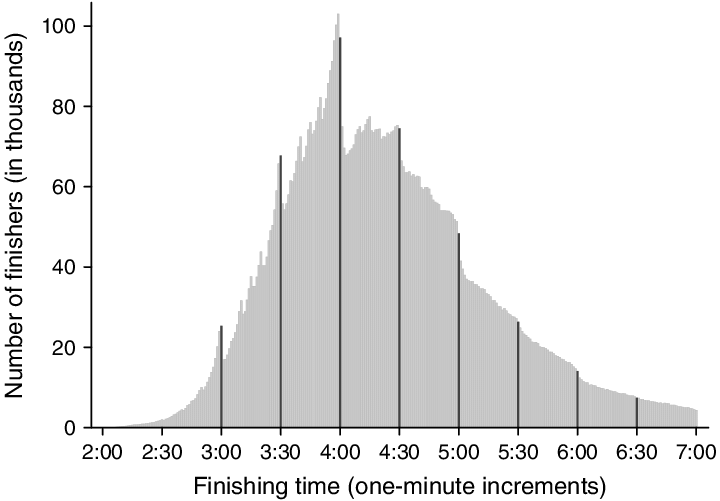
\includegraphics[width = 0.75\textwidth]{../img/marathon_finishing_times}

\vspace{5pt}
{\footnotesize Marathon finishing times. Allen et al.\ (2017), \textit{Management Science}}

\end{frame}
% ----------------------------------------------------
\note{Precise sorting. Runners speed up to finish just under 4:00, 3:30, etc. If the treatment were ``finishing under four hours'', those just below would not be comparable to those just above: they are the ones who pushed.

The standard check is to look for bunching in the distribution of the running variable at the cutoff. If people can manipulate where they land (test scores near pass marks, incomes near tax thresholds), the design breaks.}

% ----------------------------------------------------
\begin{frame}
\frametitle{What RDD needs}
\centering

\begin{itemize}
  \item<1-> No \textbf{precise sorting} around the cutoff
  \vspace{8pt}
  \item<2-> Nothing else changes at the same cutoff
  \begin{itemize}
    \item borders separate many things at once: compound treatments
  \end{itemize}
  \vspace{8pt}
  \item<3-> The estimate is \textbf{local}: it is the effect for units near the cutoff
\end{itemize}

\vspace{15pt}
\uncover<3->{{\small Variation used: the jump at the cutoff\\Must be true: \textbf{units just above and below are comparable}}}

\end{frame}
% ----------------------------------------------------
\note{The third point sets up the second half. The incumbency advantage estimated from close races tells you about close races, not about safe seats. Whether it travels is a separate argument.

Borders are popular in political science and especially tricky: a border usually bundles together laws, language, markets, media and more. Which of them is the treatment?}

% ====================================================
\section{Instrumental variables}
% ====================================================

% ----------------------------------------------------
\begin{frame}
\frametitle{Find something that moves the treatment}
\centering

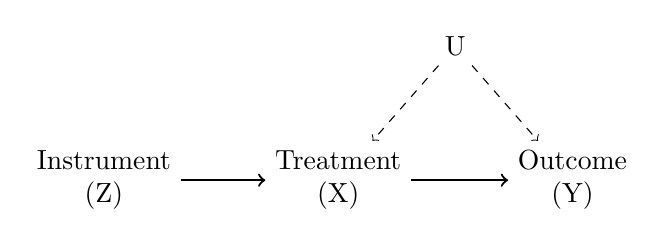
\begin{tikzpicture}[every text node part/.style={align=center}, scale = 0.85]
\node (z) at (0,0){Instrument\\(Z)};
\node (x) at (3.5,0){Treatment\\(X)};
\node (y) at (7,0){Outcome\\(Y)};
\node (u) at (5.25,2){U};
\draw[->, thick] (z) -- (x);
\draw[->, thick] (x) -- (y);
\draw[->, dashed] (u) -- (y);
\draw[->, dashed] (u) -- (x);
\end{tikzpicture}

\vspace{15pt}
\begin{itemize}
  \item A natural experiment: the coin flip, found in the wild
  \vspace{6pt}
  \item Use only the part of $X$ that is driven by $Z$
\end{itemize}

\end{frame}
% ----------------------------------------------------
\note{Same picture as the smoking coin flip at the start. The instrument does the job of the coin: it creates variation in the treatment that is unrelated to U.

The estimate comes from asking: when Z moves X, does Y move too? If Z only affects Y through X, any change in Y must be due to X.}

% ----------------------------------------------------
\begin{frame}
\frametitle{Two assumptions}
\centering

\begin{itemize}
  \item \textbf{Relevance}: $Z$ actually moves $X$
  \begin{itemize}
    \item checkable: look at the first stage
  \end{itemize}
  \vspace{12pt}
  \item<2-> \textbf{Exclusion restriction}: $Z$ affects $Y$ \textbf{only} through $X$
  \begin{itemize}
    \item no back doors from $Z$ to $Y$, and no other paths
    \item \textbf{not testable}. An argument, not a statistic
  \end{itemize}
\end{itemize}

\vspace{15pt}
\uncover<2->{
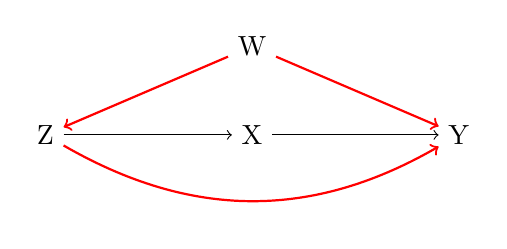
\begin{tikzpicture}[every text node part/.style={align=center}, scale = 0.75]
\node (z) at (0,0){Z};
\node (x) at (3.5,0){X};
\node (y) at (7,0){Y};
\node (w) at (3.5,1.5){W};
\draw[->] (z) -- (x);
\draw[->] (x) -- (y);
\draw[->, red, thick] (z) to [out=-30,in=-150] (y);
\draw[->, red, thick] (w) -- (z);
\draw[->, red, thick] (w) -- (y);
\end{tikzpicture}}

\end{frame}
% ----------------------------------------------------
\note{The red arrows are the two ways the exclusion restriction fails: Z has its own direct effect on Y, or Z shares a cause with Y.

The asymmetry matters: relevance can be shown with data, exclusion can only be argued. Most IV papers succeed or fail on how convincing that argument is.}

% ----------------------------------------------------
\begin{frame}
\frametitle{Example: are ethnic riots self-perpetuating?}
\centering

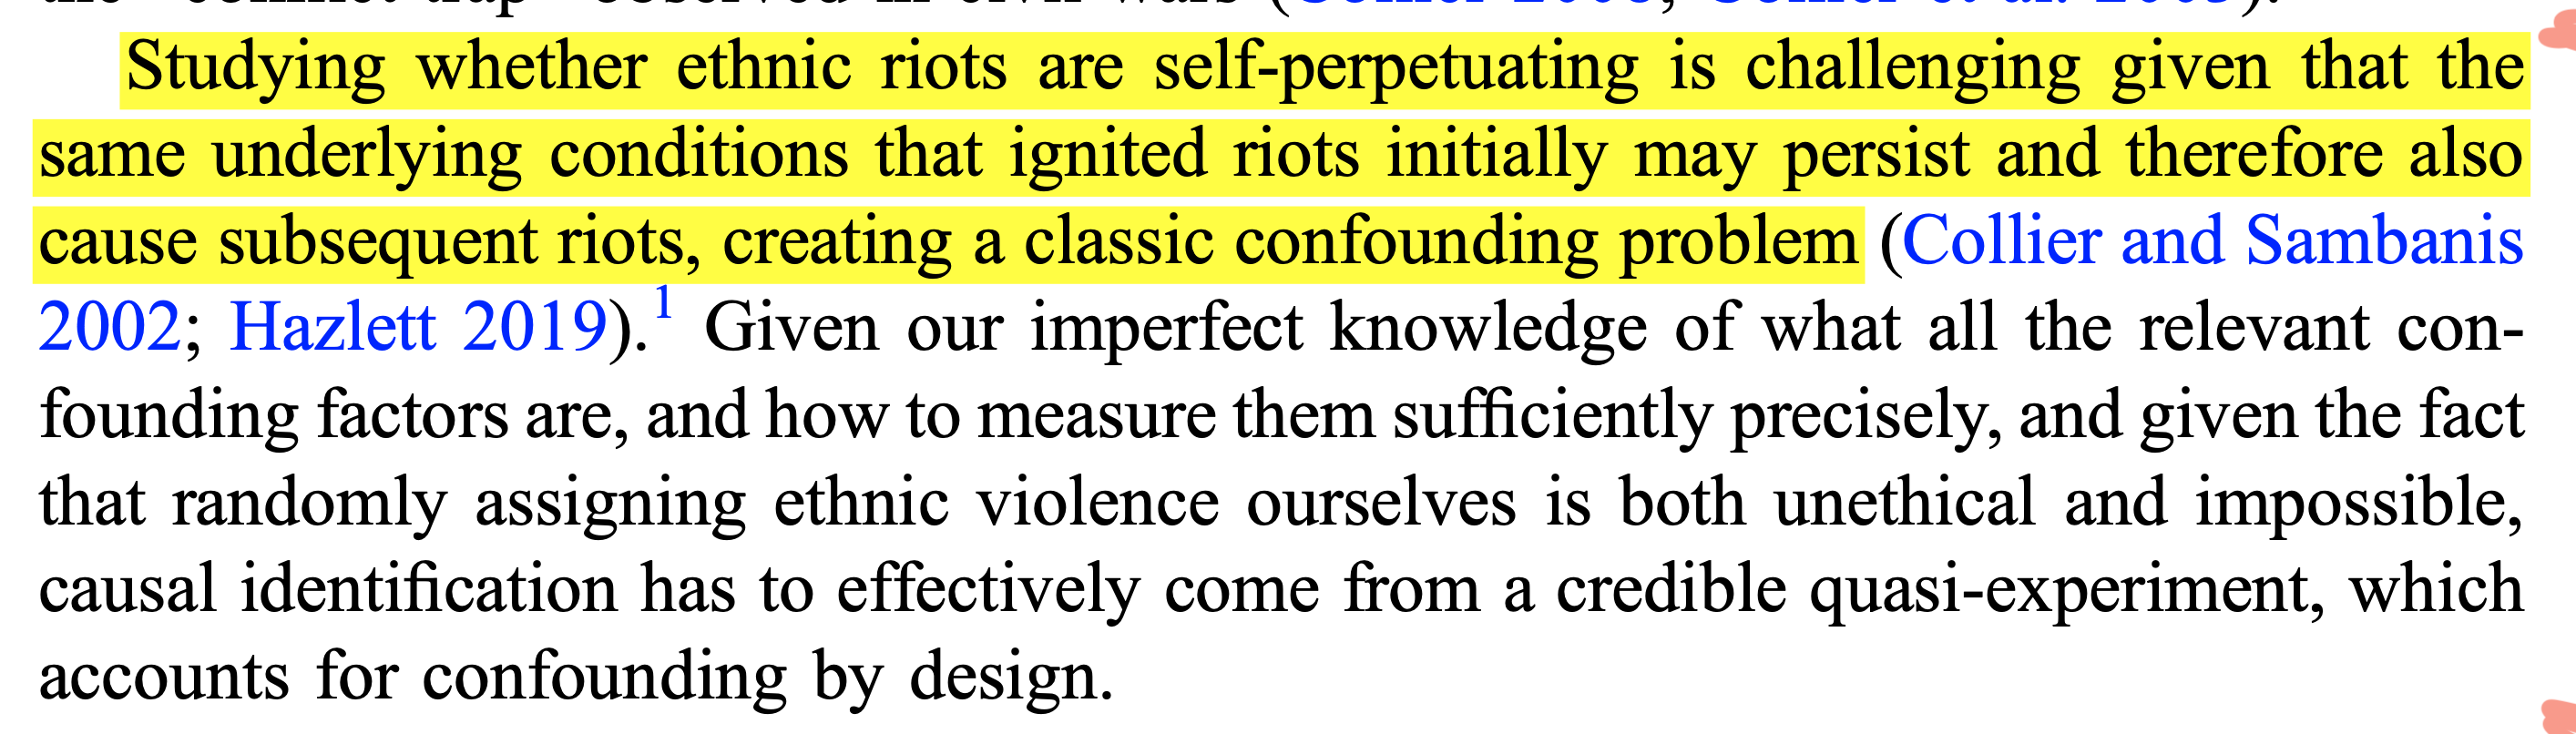
\includegraphics[width = \textwidth]{../img/india_riots3}

\vspace{5pt}
{\footnotesize van Noort \& Goyal (2025), \textit{JCR}}

\end{frame}
% ----------------------------------------------------
\note{Riots in India recur in the same places. Is that because past riots cause future ones (cycles of revenge, polarisation), or because the same underlying conditions cause both?

Ask before moving on: what could create variation in past riots that is unrelated to the local conditions that cause riots?}

% ----------------------------------------------------
\begin{frame}[plain]
  \begin{tikzpicture}[remember picture, overlay]
    \node[at = (current page.center), yshift = 0cm] (cover) {%
      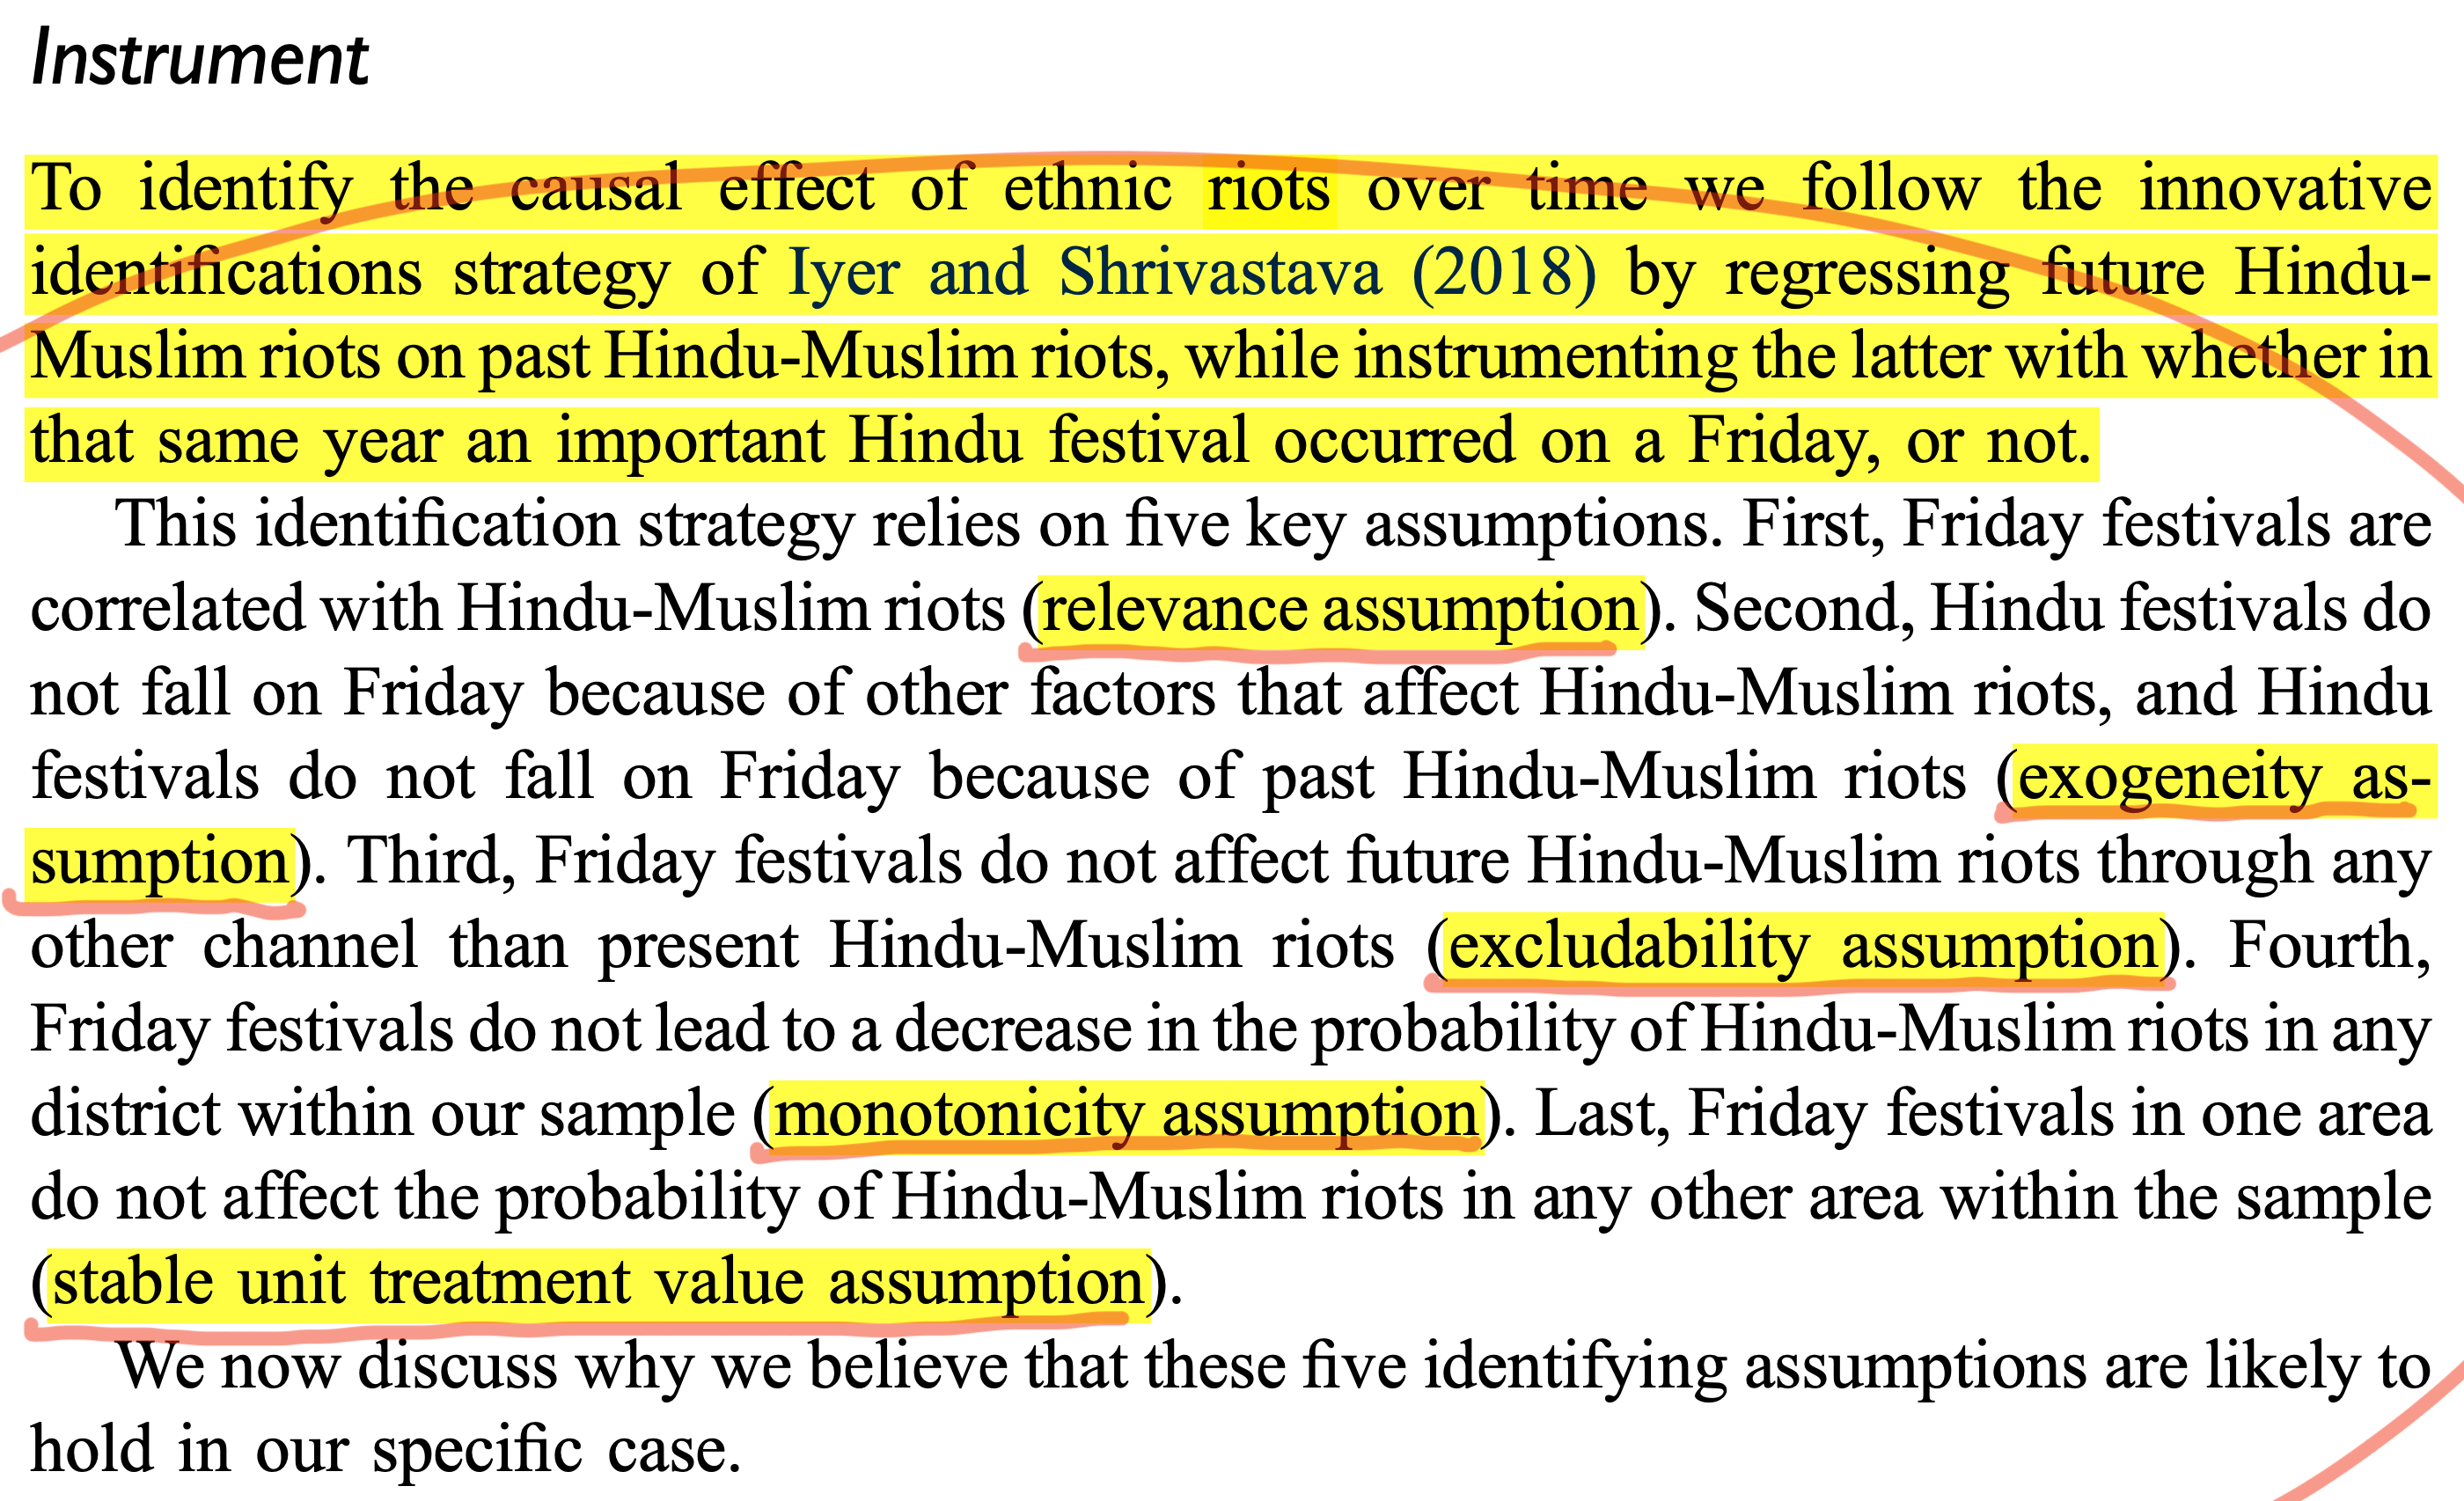
\includegraphics[keepaspectratio, width=.95\paperwidth]{../img/india_riots4}};
  \end{tikzpicture}
\end{frame}
% ----------------------------------------------------
\note{The instrument: whether an important Hindu festival falls on a Friday, the Muslim day of congregational prayer. Processions passing mosques on Fridays raise the risk of clashes. The calendar is set by lunar cycles, not by local politics.

Go through the assumptions they list. Relevance is checkable. Exclusion is the hard one: could Friday festivals affect future riots through anything other than present riots? Increased policing that year? Mobilisation that does not turn into a riot? Let students try to break it.}

% ----------------------------------------------------
\begin{frame}
\frametitle{When everyone uses the same instrument}
\centering

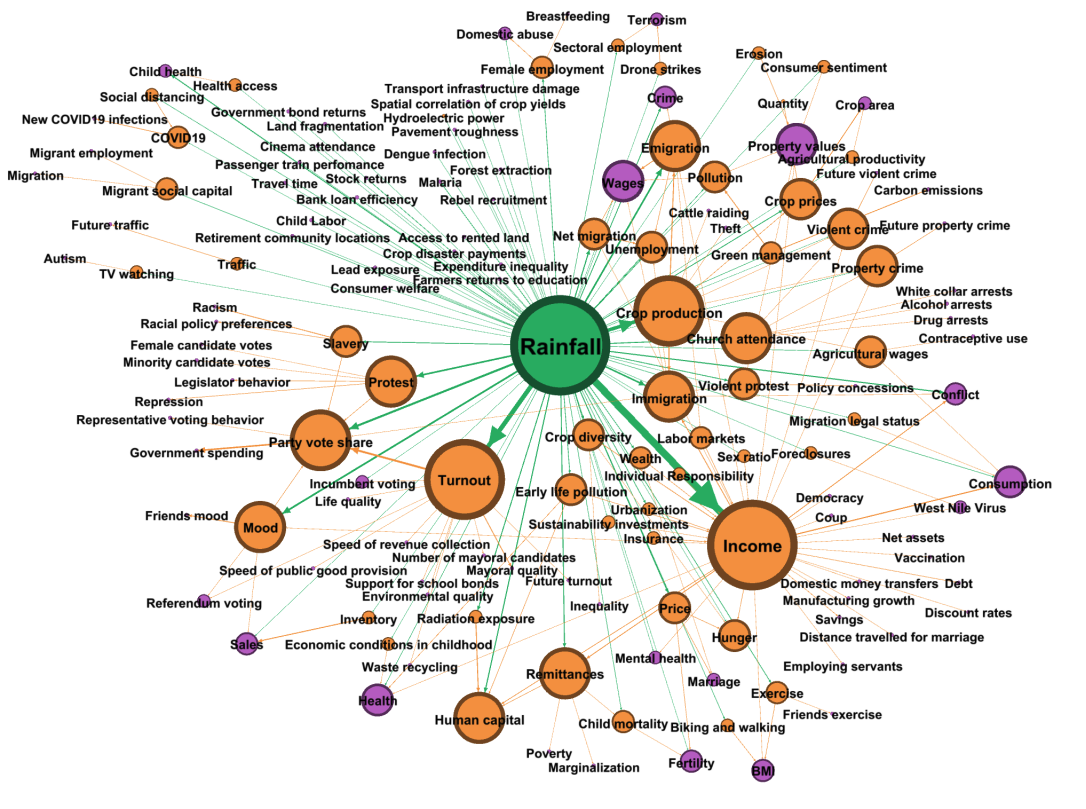
\includegraphics[keepaspectratio, width = 0.8\textwidth, height = 0.68\paperheight]{../img/rainfall_papers}

\vspace{5pt}
{\scriptsize Mellon (working paper, SSRN), ``Rain, Rain, Go Away: 192 Potential Exclusion-Restriction Violations for Studies Using Weather as an Instrumental Variable''}

\end{frame}
% ----------------------------------------------------
\note{Rainfall has been used as an instrument for income, conflict, protest, turnout, migration and much else. Each paper argues that rain only affects its outcome through its own treatment.

But if rain affects income, and turnout, and protest, then a paper using rain as an instrument for income in a model of protest violates the exclusion restriction through all the other channels. Every new paper that ``validates'' rain as an instrument for X undermines every other paper using it for something else.

Lesson: an instrument is only as good as the argument that it has no other paths, and those arguments do not stack.}

% ----------------------------------------------------
\begin{frame}
\frametitle{What IV needs}
\centering

\vspace{10pt}
\begin{itemize}
  \item A \textbf{relevant} instrument
  \vspace{8pt}
  \item A believable \textbf{exclusion restriction}
  \vspace{8pt}
  \item<2-> Also local: the effect is for units whose treatment \textbf{responds to the instrument}
  \begin{itemize}
    \item the LATE, or effect on ``compliers''
  \end{itemize}
\end{itemize}

\vspace{15pt}
\uncover<2->{{\small Variation used: the part of $X$ driven by $Z$\\Must be true: \textbf{$Z$ affects $Y$ only through $X$}}}

\end{frame}
% ----------------------------------------------------
\note{The LATE point again, as with RDD. In the riots paper, the effect is for districts where Friday festivals tip things into riots. Are those typical districts? Probably they are the most tense ones.

This is a recurring trade-off: the cleaner the identification, the narrower the population the estimate is about.}

% ====================================================
\section{Putting it together}
% ====================================================

% ----------------------------------------------------
\begin{frame}
\frametitle{The templates in one table}
\centering

\footnotesize
\renewcommand{\arraystretch}{1.5}
\begin{tabular}{>{\raggedright\arraybackslash}p{2cm}>{\raggedright\arraybackslash}p{3.2cm}>{\raggedright\arraybackslash}p{3.4cm}}
\hline
\textbf{Design} & \textbf{Variation used} & \textbf{Must be true} \\
\hline
Controls, matching & Treated vs.\ untreated who look alike & No unobserved confounders \\
Fixed effects & Within groups & No confounders varying within groups \\
\hline
DiD & Change over time, treated vs.\ untreated & Parallel trends \\
RDD & Jump at a cutoff & No sorting, nothing else at the cutoff \\
IV & Part of $X$ moved by $Z$ & Exclusion restriction \\
\hline
\end{tabular}

\end{frame}
% ----------------------------------------------------
\note{The summary slide to photograph. If their workshop presentation can fill one row of this table for their own project, the comparison part of the design is done.

Note that none of the right-hand column is fully testable. Each design trades one untestable assumption for another, hopefully more plausible, one.}

% ----------------------------------------------------
\begin{frame}
\frametitle{Combining: does pollution make people leave the city?}
\centering

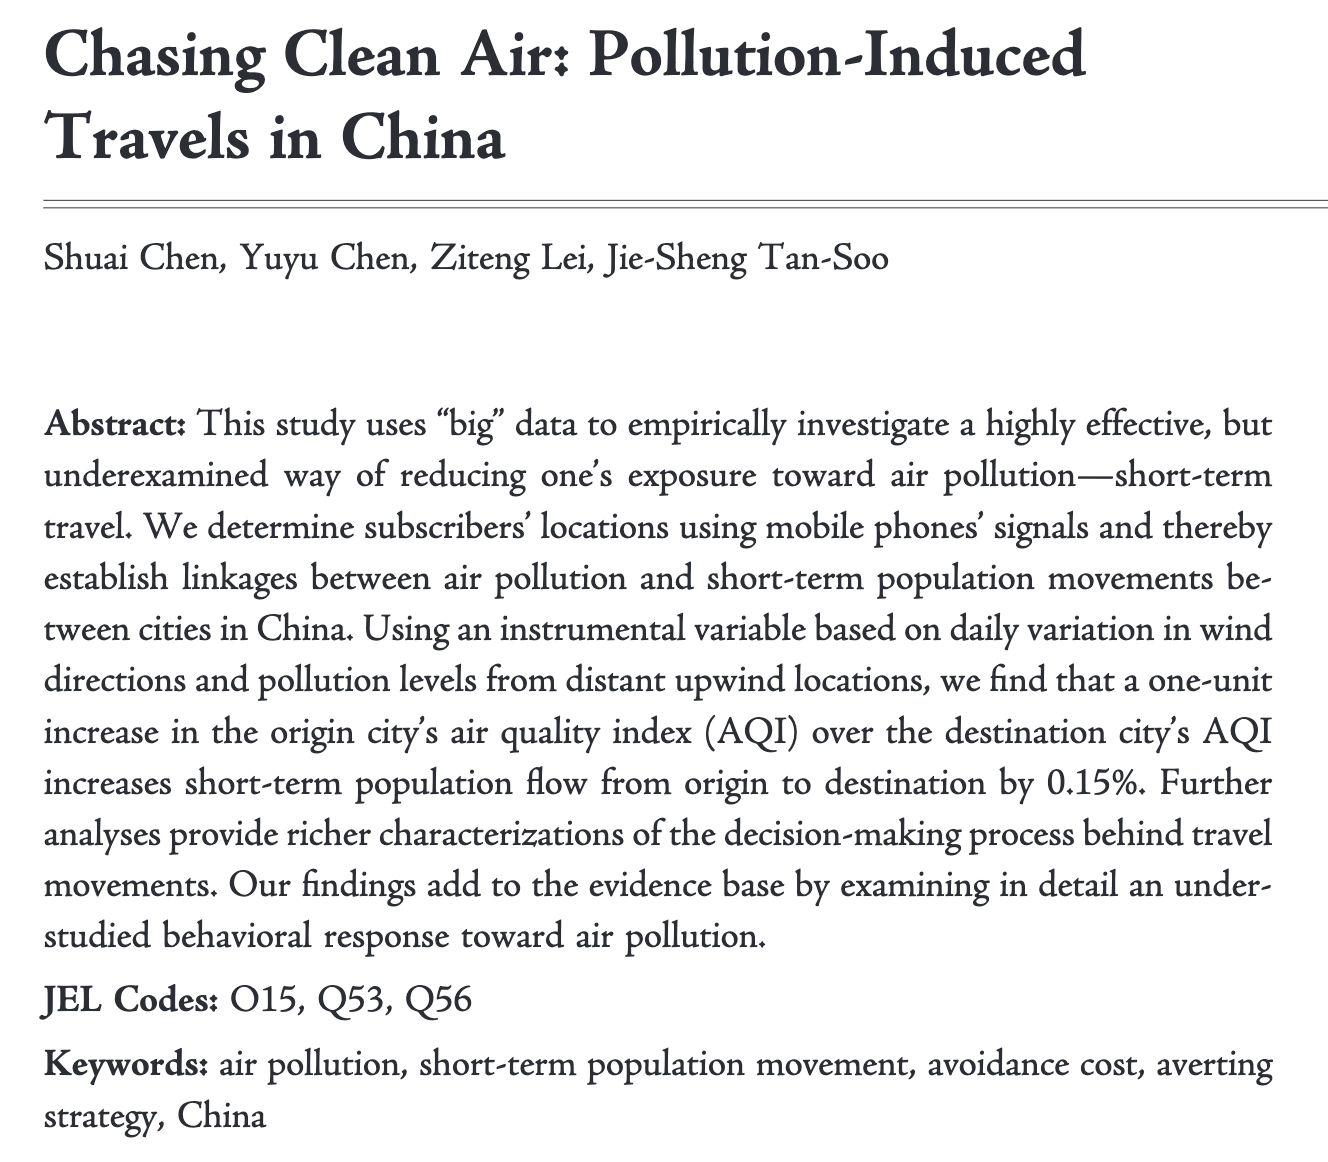
\includegraphics[width = 0.65\textwidth]{../img/china_pollution}

\vspace{5pt}
{\footnotesize Chen, Chen, Lei \& Tan-Soo (2021), \textit{JAERE}}

\end{frame}
% ----------------------------------------------------
\note{A computational example: phone location data for short-term travel between Chinese cities. Pollution is obviously endogenous to economic activity and traffic, which also drive travel.

The instrument: daily wind direction carrying pollution from distant upwind locations. Ask: is wind direction enough on its own?}

% ----------------------------------------------------
\begin{frame}
\frametitle{Combining: does pollution make people leave the city?}
\centering

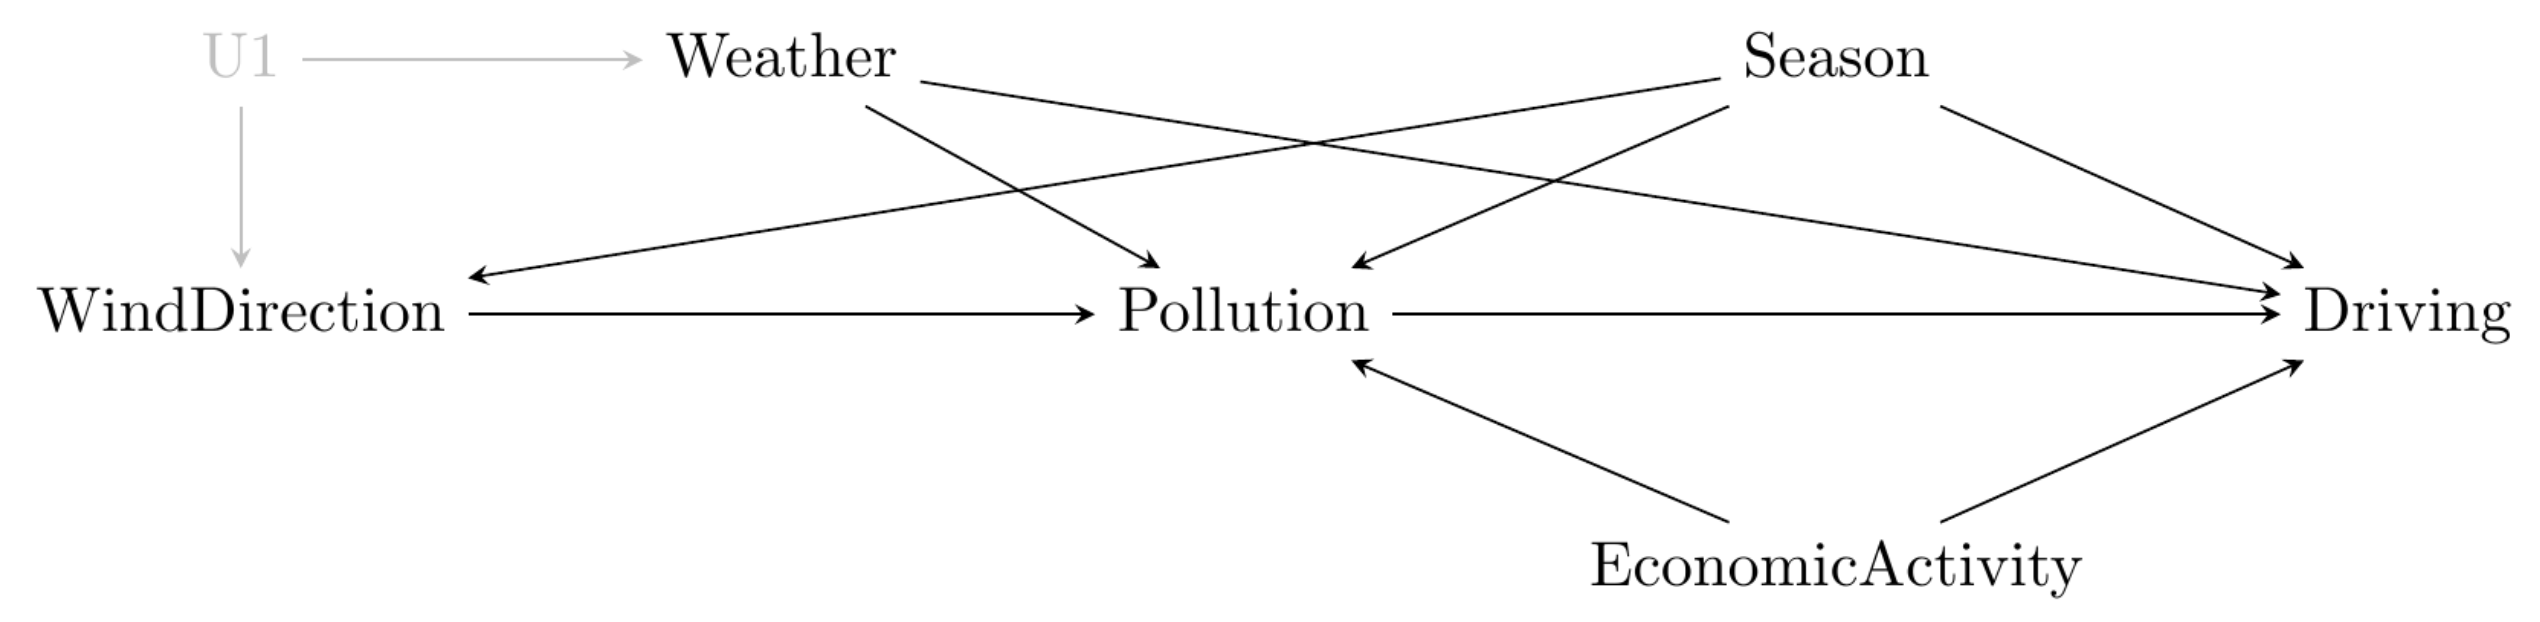
\includegraphics[width = \textwidth]{../img/china_pollution_dag}

\vspace{15pt}
\begin{itemize}
  \item<2-> Wind direction is linked to \textbf{weather and season}, which also affect travel
  \item<2-> So: instrument with wind, \textbf{and} control for weather, season and city
\end{itemize}

\end{frame}
% ----------------------------------------------------
\note{This is what real designs look like. The instrument is only valid conditional on weather, season and city, so the paper exploits exogenous variation and closes the remaining back doors at the same time.

Back to the opening: most good papers do both.}

% ----------------------------------------------------
\begin{frame}
\frametitle{In pairs: which template?}
\centering

\vspace{5pt}
\small
\begin{enumerate}
  \item Do Airbnb listings raise rents in a neighbourhood?
  \vspace{8pt}
  \item Does content moderation reduce hate speech on a platform?
  \vspace{8pt}
  \item Does having a female mayor change local spending?
  \vspace{8pt}
  \item Does exposure to cross-cutting news reduce polarization?
\end{enumerate}

\vspace{10pt}
{\footnotesize For each: what variation would you use, and what has to be true?}

\end{frame}
% ----------------------------------------------------
\note{Ten minutes, then cold-call one pair per question. There is no single right answer; what matters is that they name the variation and the assumption.
\begin{enumerate}
  \item DiD with staggered entry of Airbnb into neighbourhoods; or an IV based on distance to tourist sites interacted with the global rise of the platform. Threat: Airbnb goes where gentrification is already happening.
  \item DiD around a moderation policy change, comparing affected and unaffected communities or languages. Threat: users move to other platforms, so the outcome is displaced, not reduced.
  \item RDD on close mixed-gender elections. Threat: the effect is local to competitive races.
  \item Field experiment if possible; otherwise fixed effects on panel data of users. Threat: who chooses to read cross-cutting news.
\end{enumerate}}

% ----------------------------------------------------
\begin{frame}
\frametitle{}
\centering

\vspace{40pt}
{\Large Break}

\vspace{10pt}
{\small 10 minutes}

\end{frame}
% ----------------------------------------------------
\note{Halfway point. If running late, the slides on staggered DiD, the funnel plots and the second meta-analysis slide can be skipped without losing the thread.}

% ====================================================
\section{How far does it travel?}
% ====================================================

% ----------------------------------------------------
\begin{frame}
\frametitle{Credible here, but where else?}
\centering

\begin{itemize}
  \item \textbf{Internal validity}: is the effect real \textit{here}?
  \vspace{8pt}
  \item The \textbf{credibility revolution}: designs with strong internal validity, usually in a specific place and time
  \vspace{8pt}
  \item<2-> The cost: the cleanest designs answer narrow questions
  \begin{itemize}
    \item close elections, compliers, one border, one platform, one year
  \end{itemize}
  \vspace{8pt}
  \item<3-> Every step from topic to question to measure to design \textbf{loses something}
  \vspace{8pt}
  \item<4-> So: what have we learned about the \textbf{big question}?
\end{itemize}

\end{frame}
% ----------------------------------------------------
\note{Second half. Everything so far was about internal validity: is the effect real \textbf{here}? Now: what does it tell us beyond here?

Connect to session 2: they narrowed big topics into answerable questions. That was necessary. The cost shows up now, when they have to explain what the narrow answer says about the broad topic.}

% ----------------------------------------------------
\begin{frame}
\frametitle{Three kinds of validity beyond ``here''}
\centering

\begin{itemize}
  \item \textbf{Construct validity}: is the treatment really the cause you name? Is the outcome really what you mean?
  \vspace{10pt}
  \item \textbf{External validity}: would it hold for other people, treatments, outcomes, places?
  \vspace{10pt}
  \item \textbf{Temporal validity}: would it still hold now?
\end{itemize}

\end{frame}
% ----------------------------------------------------
\note{Three questions to ask of any result, including their own. One slide each.}

% ----------------------------------------------------
\begin{frame}
\frametitle{Construct validity}
\centering

\begin{itemize}
  \item About \textbf{mislabeling} the cause or the outcome
  \vspace{8pt}
  \item Of the cause: \textbf{bundled treatments}
  \begin{itemize}
    \item Guess et al.: the chronological feed changed political content, untrustworthy content, incivility, \textit{and} time on platform
    \item a border is laws, language, markets and media at once
  \end{itemize}
  \vspace{8pt}
  \item<2-> Of the outcome: session 3 again
  \begin{itemize}
    \item does your measure of polarization capture polarization?
  \end{itemize}
\end{itemize}

\end{frame}
% ----------------------------------------------------
\note{Guess et al.\ is the perfect example because they read it last week. The randomization was perfect, so the effect of ``the chronological feed'' is well identified. But what is the chronological feed, as a cause? It is a bundle. Saying ``algorithms do not affect polarization'' relabels it.

Link to session 3: construct validity of the outcome is the measurement problem, seen from the end of the project.}

% ----------------------------------------------------
\begin{frame}
\frametitle{External validity}
\centering

\begin{itemize}
  \item Unlikely that any effect holds under all conditions. The question is \textbf{under which}
  \vspace{8pt}
  \item Generalize to other\ldots
  \begin{itemize}
    \item \textbf{units} (who was studied?)
    \item \textbf{treatments} (a different dose or version?)
    \item \textbf{outcomes} (a different measure?)
    \item \textbf{contexts} (another country, platform, period?)
  \end{itemize}
  \vspace{8pt}
  \item<2-> Generalizing the \textbf{sign} is easier than the \textbf{size}
\end{itemize}

\vspace{5pt}
{\footnotesize \asher{Egami \& Hartman (2023), \textit{APSR}}}

\end{frame}
% ----------------------------------------------------
\note{Egami and Hartman's framework (X-, T-, Y- and C-validity). The useful point for design: external validity is not a vague worry to mention in the conclusion. You can design for it, by sampling diverse contexts or by theorising which conditions should matter and testing for heterogeneity.

Sign- versus effect-generalization: ``this kind of intervention reduces X'' is often defensible when ``by 3 points'' is not.}

% ----------------------------------------------------
\begin{frame}
\frametitle{Temporal validity}
\centering

\begin{itemize}
  \item ``All of the knowledge contained in published papers comes from the past, and all action is in the future''
  \vspace{8pt}
  \item<2-> Knowledge \textbf{decays}, at a rate that depends on how fast the world changes
  \vspace{8pt}
  \item<3-> In computational social science, that rate is high
  \begin{itemize}
    \item what do we know about Twitter that holds for X?
    \item platforms change their algorithms, users, and rules continuously
  \end{itemize}
\end{itemize}

\vspace{10pt}
{\footnotesize \asher{Munger (2023), \textit{Research \& Politics}}}

\end{frame}
% ----------------------------------------------------
\note{This one is especially for them. Munger's argument: the incremental model of science (accumulate well-identified effects) assumes the world stands still while we accumulate. When it changes fast, studies go out of date before they replicate.

Drift from session 2 is the same problem seen from the data side: the data-generating process changes under you. Google Flu again.

Not a reason for despair, but for theory: knowing \textbf{why} an effect occurred is what lets you guess whether it survives a change.}

% ----------------------------------------------------
\begin{frame}
\frametitle{Learning across studies: meta-analysis}
\centering

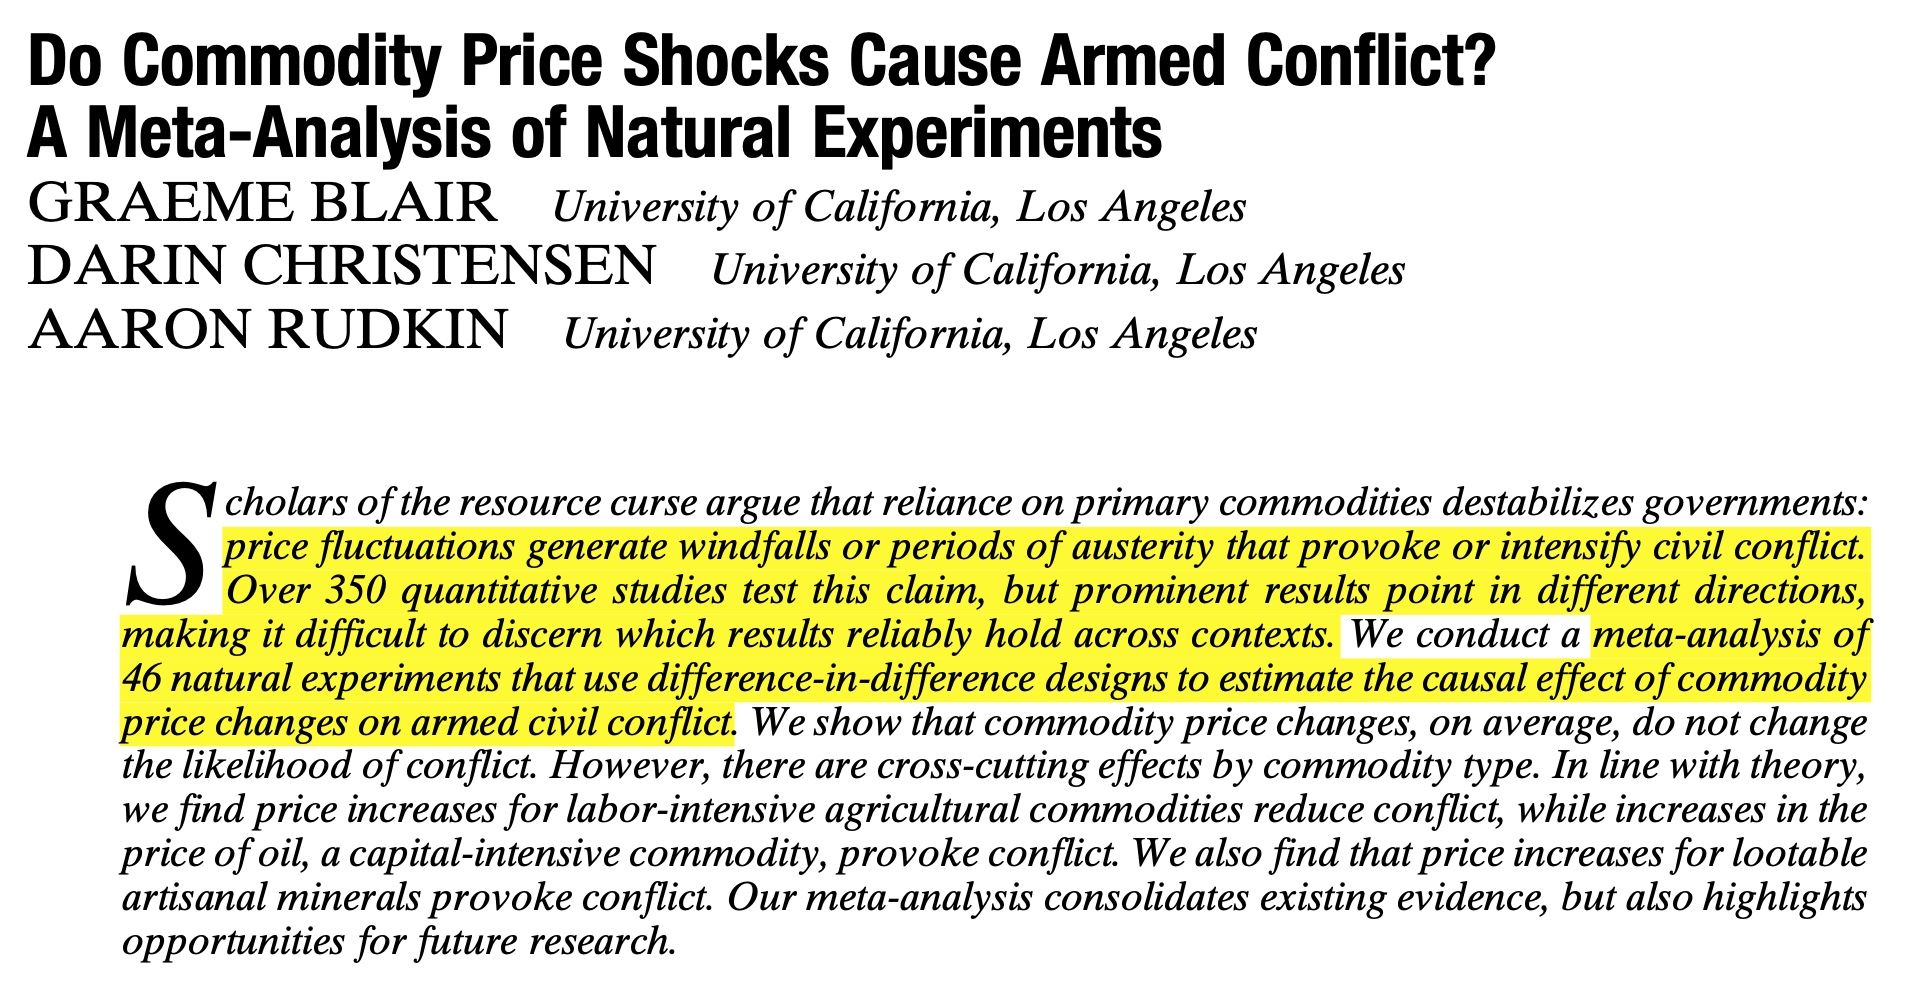
\includegraphics[width = 0.9\textwidth]{../img/blair_apsr}

\vspace{5pt}
\begin{itemize}
  \item Do commodity price shocks cause conflict? 46 studies, same design
\end{itemize}

\end{frame}
% ----------------------------------------------------
\note{Blair, Christensen and Rudkin (2021). Natural resources and conflict is a classic endogeneity problem: resource-rich countries differ in many ways.

The design that many papers converged on: world commodity prices are exogenous to any one country's conflict, so price shocks interacted with a country's production give a DiD-type design with country and year fixed effects. The meta-analysis pools 46 such studies.}

% ----------------------------------------------------
\begin{frame}
\frametitle{What the meta-analysis found}
\centering

\begin{itemize}
  \item Pooling all commodities: \textbf{no effect}
  \vspace{8pt}
  \item<2-> Split by type, as theory predicts:
  \begin{itemize}
    \item agricultural prices up $\rightarrow$ \textbf{less} conflict (opportunity cost of fighting)
    \item oil and gas prices up $\rightarrow$ \textbf{more} conflict (bigger prize)
  \end{itemize}
  \vspace{8pt}
  \item<3-> Also shows the \textbf{gaps}: where and when the evidence comes from, and what goes unpublished
\end{itemize}

\end{frame}
% ----------------------------------------------------
\note{The punchline: the pooled null hides two opposite effects. Without theory telling you to split labour-intensive from capital-intensive commodities, you would conclude that prices don't matter.

Same lesson as external validity: an average effect is only meaningful if the units are similar in the ways that matter. That leads into the next section, on what does not get published.}

% ====================================================
\section{Keeping yourself honest}
% ====================================================

% ----------------------------------------------------
\begin{frame}[plain]
  \begin{tikzpicture}[remember picture, overlay]
    \node[at = (current page.center), yshift = 0cm] (cover) {%
      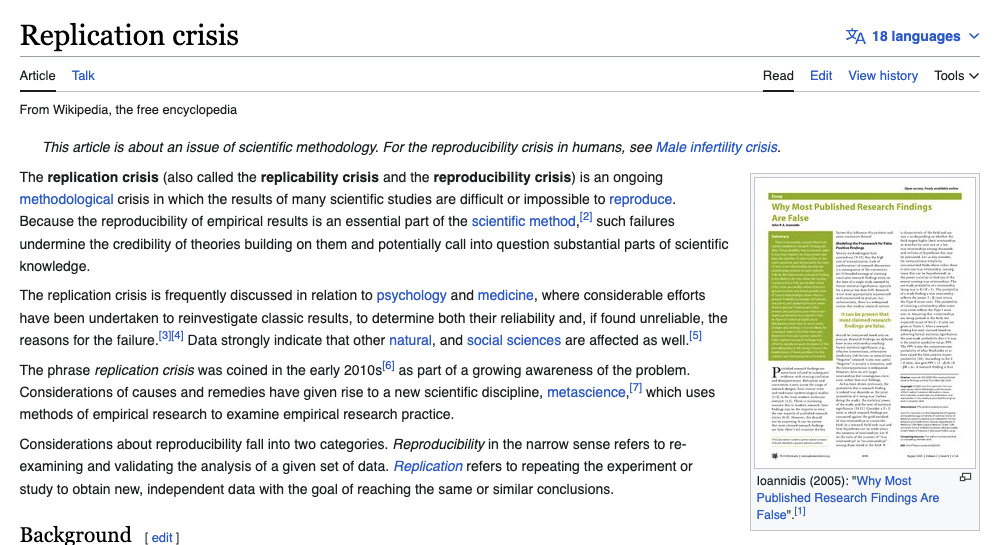
\includegraphics[keepaspectratio, width=.95\paperwidth]{../img/replicationcrisis1}};
  \end{tikzpicture}
\end{frame}
% ----------------------------------------------------
\note{Many published findings, especially in psychology but also elsewhere, do not replicate. Ioannidis (2005) argued that most published research findings are false.

The causes are not mainly fraud. They are design and incentive problems: small samples, flexible analyses, and journals that prefer positive results. The next slides are about the design side.}

% ----------------------------------------------------
\begin{frame}
\frametitle{Researcher degrees of freedom}
\centering

\begin{itemize}
  \item Every project involves dozens of reasonable decisions
  \begin{itemize}
    \item which outcome, which measure, which controls, which sample, which period, which estimator
  \end{itemize}
  \vspace{8pt}
  \item<2-> Each choice made \textbf{after seeing the results} tilts them
  \begin{itemize}
    \item no bad intentions needed: the ``garden of forking paths''
  \end{itemize}
  \vspace{8pt}
  \item<3-> Worse with big data: more variables, more subgroups, more ways to slice
\end{itemize}

\end{frame}
% ----------------------------------------------------
\note{Gelman and Loken's ``garden of forking paths'': even a researcher who runs only one analysis can be biased if the choice of that analysis depended on the data.

The CSS point: big data does not fix this, it amplifies it. With millions of observations everything is statistically significant, and with hundreds of possible features there are endless defensible specifications.}

% ----------------------------------------------------
\begin{frame}
\frametitle{Publication bias leaves a trace}
\centering

\begin{minipage}{0.48\textwidth}\centering
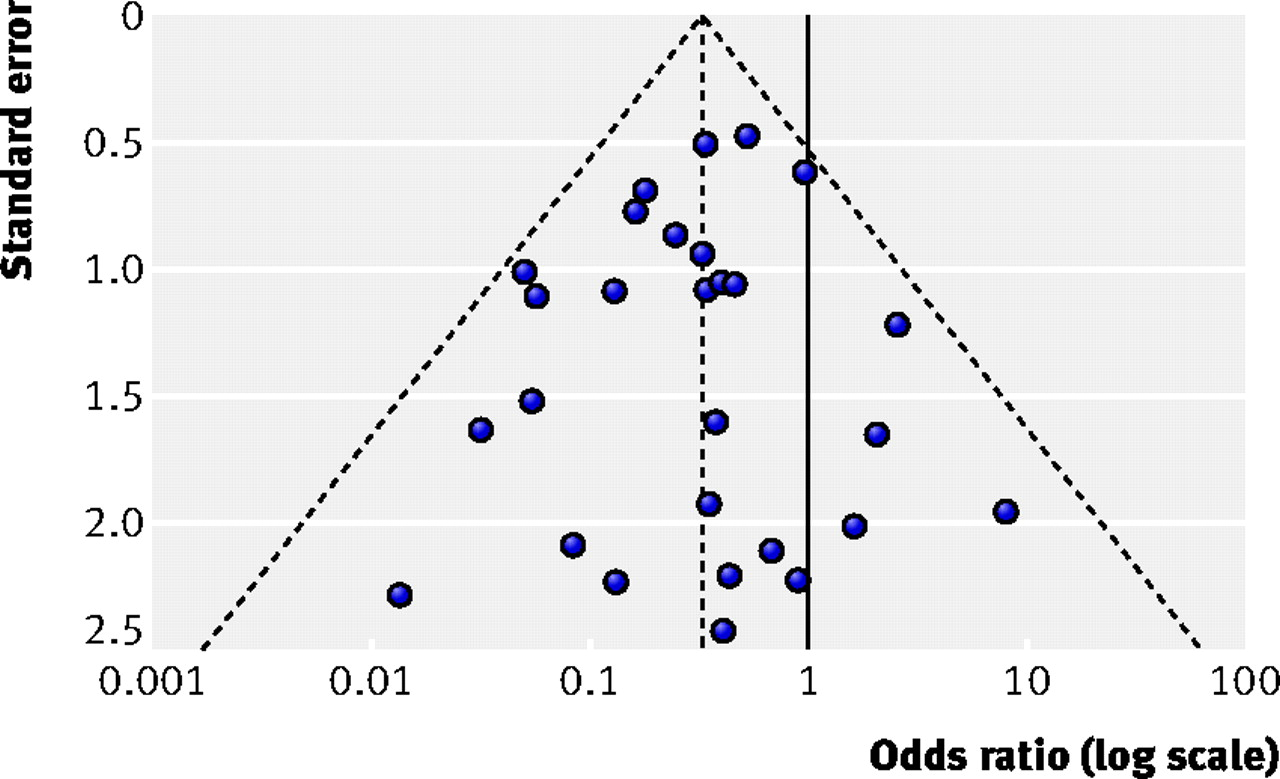
\includegraphics[width = \textwidth]{../img/funnel_good}\\
{\footnotesize No bias}
\end{minipage}\hfill
\begin{minipage}{0.48\textwidth}\centering
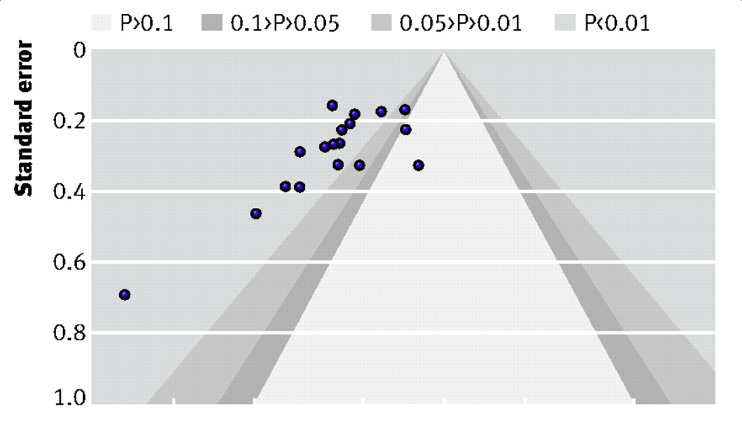
\includegraphics[width = \textwidth]{../img/funnel_bad}\\
{\footnotesize Bias}
\end{minipage}

\vspace{15pt}
{\small Funnel plots: effect size vs.\ precision across studies.\\ Imprecise studies should scatter on \textbf{both} sides of the truth}

\end{frame}
% ----------------------------------------------------
\note{(Optional, skip if short of time.) How meta-analyses detect publication bias. Precise studies (top) cluster around the true effect. Imprecise ones (bottom) should scatter widely on both sides. If one bottom corner is empty, small studies with the ``wrong'' or null result were never published.

Caveat: asymmetry can also reflect real heterogeneity between studies, not only publication bias.}

% ----------------------------------------------------
\begin{frame}
\frametitle{Two responses}
\centering

\begin{itemize}
  \item \textbf{Pre-registration} and \textbf{pre-analysis plans}
  \begin{itemize}
    \item write down hypotheses, measures and analyses \textit{before} seeing outcomes
    \item what you did not pre-register is still allowed, but labelled exploratory
  \end{itemize}
  \vspace{10pt}
  \item<2-> \textbf{Robustness} as design logic
  \begin{itemize}
    \item which reasonable choices could change the result? Show them all
  \end{itemize}
  \vspace{10pt}
  \item<3-> Your final essay can be a pre-analysis plan
\end{itemize}

\end{frame}
% ----------------------------------------------------
\note{Guess et al.\ was pre-registered, which is part of why a null result from it is credible and publishable.

Pre-registration for observational and found data is harder (the data often already exists), but the logic still applies: commit to the design before looking at the outcome.

The last point is a direct link to their assessment. A pre-analysis plan is exactly what the essay can be: the design, written down before the data.}

% ----------------------------------------------------
\begin{frame}
\frametitle{Placebo tests: look where there should be nothing}
\centering

\begin{itemize}
  \item If your design is right, some things should \textbf{not} happen
  \vspace{6pt}
  \item Example: Russian TV signal strength and voting in Ukraine
  \vspace{6pt}
  \item<2->[1.] \textbf{Placebo outcome}: signal should not predict things it can't affect (pre-existing share of Russian speakers)
  \vspace{4pt}
  \item<3->[2.] \textbf{Placebo treatment}: signal of Russian \textit{sports} channels should not predict voting
  \vspace{4pt}
  \item<4->[3.] \textbf{Placebo population}: no effect among satellite TV users, for whom signal is irrelevant
\end{itemize}

\vspace{8pt}
{\footnotesize \asher{Peisakhin \& Rozenas (2018), \textit{AJPS}; Eggers, Tuñón \& Dafoe (2024), \textit{AJPS}}}

\end{frame}
% ----------------------------------------------------
\note{Placebo tests are design logic, not statistical decoration. Each one asks: if the alternative explanation were true, what would we see? Then looks.

They have already seen two placebo tests today: pre-trends in DiD (a placebo period) and the balance test at the Pale border in Boix (placebo outcomes). The Russian TV example shows all three types cleanly.

For the essay: every design should come with at least one ``this should not happen'' test.}

% ====================================================
\section{Ethics for computational work}
% ====================================================

% ----------------------------------------------------
\begin{frame}
\frametitle{An experiment on 689,000 people}
\centering

\begin{itemize}
  \item Facebook, 2012: reduced positive or negative posts in users' feeds for a week
  \vspace{6pt}
  \item Outcome: the emotional tone of what users then posted
  \vspace{6pt}
  \item Published in \textit{PNAS} (Kramer, Guillory \& Hancock 2014)
  \vspace{6pt}
  \item<2-> No specific consent. Justified by the terms of service
  \vspace{6pt}
  \item<3-> Same platform, same kind of intervention as Guess et al. What is different?
\end{itemize}

\end{frame}
% ----------------------------------------------------
\note{The emotional contagion study. The effects were tiny, the backlash was huge. Ask the closing question openly and give it a couple of minutes.

Differences with Guess et al.: explicit consent to participate, ethics review, compensation, pre-registration, academic control over the analysis. Similarities: the platform still controlled access and the intervention, and the participants were a selected group.}

% ----------------------------------------------------
\begin{frame}
\frametitle{Questions that design raises}
\centering

\begin{itemize}
  \item \textbf{Consent}: accepting terms of service is not consenting to research
  \vspace{8pt}
  \item \textbf{Harm}: would anyone be worse off because of your study?
  \vspace{8pt}
  \item \textbf{Re-identification}: ``anonymised'' traces often aren't
  \vspace{8pt}
  \item \textbf{Legality}: scraping, platform rules, data protection
\end{itemize}

\vspace{10pt}
{\footnotesize \asher{Salganik, \textit{Bit by Bit}, ch.\ 6: respect for persons, beneficence, justice, respect for law and public interest}}

\end{frame}
% ----------------------------------------------------
\note{Salganik's four principles are the framework to cite in the essay. The practical point: ethics is a design constraint, not an appendix. Many of the cleanest designs (randomising exposure to harmful content, scraping private groups) are off the table for ethical reasons, and that shapes which question you can answer.

Re-identification: the Netflix Prize data and the AOL search logs are the classic cases. A few behavioural traces are enough to identify a person.}

% ====================================================
\section{Wrapping up}
% ====================================================

% ----------------------------------------------------
\begin{frame}
\frametitle{What credibility means for each goal}
\centering

\vspace{10pt}
\begin{itemize}
  \item \textbf{Describe}: coverage, a defensible denominator, a clear population
  \vspace{10pt}
  \item \textbf{Explain}: a comparison whose assumption you can defend
  \vspace{10pt}
  \item \textbf{Predict}: performance on data the model has not seen, \textit{from the future}
\end{itemize}

\vspace{15pt}
\uncover<2->{{\small All three: \textbf{how far does it travel?}}}

\end{frame}
% ----------------------------------------------------
\note{Closing the loop on session 1. Each goal has its own standard of credibility, and today was mostly about the second.

On prediction: out-of-sample testing is the equivalent of identification, but random train/test splits are not enough when the world drifts. Test on later data. Watch for leakage (features that encode the outcome). Google Flu fails exactly here.

The last line is common to the three: description of one platform, an effect at one border, a model trained on one year. All face the same question about how far they travel.}

% ----------------------------------------------------
\begin{frame}
\frametitle{In your groups: twenty minutes}
\centering

\vspace{10pt}
\begin{enumerate}
  \item Say your question in one sentence. Which goal?
  \vspace{8pt}
  \item Which \textbf{row of the table} is your design?
  \vspace{8pt}
  \item What has to be true? How would you check it?
  \vspace{8pt}
  \item Which threat will you \textbf{not} be able to solve?
\end{enumerate}

\vspace{15pt}
{\small I'll come round. No group yet? Use this to find one}

\end{frame}
% ----------------------------------------------------
\note{The working part of the session. Twenty minutes in groups while I go table to table, then two or three groups share their design in two minutes each for feedback from the room.

Students without a group: put them together in this activity. Groups are fixed by the Memo 5 deadline.

Watch for the usual problems: questions that are topics, designs that are a list of methods, ``we will control for everything'', and predictive models presented as causal.}

% ====================================================
\section{Memo 5, workshop and essay}
% ====================================================

% ----------------------------------------------------
\begin{frame}
\frametitle{One project, seen three times}
\centering

\vspace{15pt}
\begin{tikzpicture}[scale = 1]
  % period bands
  \fill[accent!25] (0,-0.25) rectangle (3.6,-0.75);
  \fill[accent2!25] (3.6,-0.25) rectangle (8.4,-0.75);
  \fill[yellow!50] (8.4,-0.25) rectangle (9.6,-0.75);
  \node[font=\scriptsize] at (1.8,-0.5) {design};
  \node[font=\scriptsize] at (6,-0.5) {write the essay};
  \node[font=\scriptsize, align=center] at (9.0,-1.1) {revise};
  % line
  \draw[thick, ->] (-0.3,0) -- (10,0);
  % ticks
  \draw[thick] (0,0) -- (0,1.4);
  \node[font=\scriptsize, align=center, above] at (0,1.4) {\textbf{Today}\\Oct 13};
  \draw[thick] (3.6,0) -- (3.6,0.6);
  \node[font=\scriptsize, align=center, above] at (3.6,0.6) {\textbf{Memo 5}\\Mon Oct 19};
  \draw[thick] (8.4,0) -- (8.4,1.4);
  \node[font=\scriptsize, align=center, above] at (8.4,1.4) {\textbf{Workshop}\\Mon Oct 26};
  \draw[thick] (9.6,0) -- (9.6,0.6);
  \node[font=\scriptsize, align=center, above] at (9.6,0.6) {\textbf{Essay}\\Oct 27};
\end{tikzpicture}

\vspace{20pt}
\footnotesize
\begin{tabular}{lrl}
\hline
Design memos (5) & 15\% & the pair (Memo 5: the group) \\
Workshop presentation & 35\% & the group \\
Workshop feedback & 10\% & the group \\
Final essay & 40\% & the group \\
\hline
\end{tabular}

\end{frame}
% ----------------------------------------------------
\note{The big picture first. Memo 5, the presentation, the feedback and the essay are the same project at three moments. That is why the group is the same for all of them.

85\% of the grade is group work from here on. Two weeks left: one to settle the design, one to write.}

% ----------------------------------------------------
\begin{frame}
\frametitle{Memo 5: the design on one page}
\centering

\begin{itemize}
  \item Written by your \textbf{workshop group} (3--4 people), not in pairs
  \vspace{4pt}
  \item Due \textbf{Monday Oct 19}, Aula Global, by midnight
  \vspace{8pt}
  \item<2-> One page, six items:
  \begin{itemize}
    \item goal $\cdot$ question $\cdot$ units and variation
    \item measure $\cdot$ comparison $\cdot$ the threat you cannot solve
  \end{itemize}
  \vspace{8pt}
  \item<3-> Whoever submits together \textbf{is a group}: binding for the presentation and the essay
  \vspace{4pt}
  \item<3-> It goes to your \textbf{paired group}, who use it to prepare
\end{itemize}

\end{frame}
% ----------------------------------------------------
\note{The six items are the same as the presentation and the essay. If Memo 5 is done properly, the skeleton of the essay exists by Monday.

Graded lightly like the other memos (done, or done well). The real function is to fix the groups and give the paired group a head start.

Anyone still without a group should talk to me today, not on Monday night.}

% ----------------------------------------------------
\begin{frame}
\frametitle{What your presentation should cover}
\centering

\begin{itemize}
  \item The \textbf{goal}: describe, explain, or predict?
  \vspace{4pt}
  \item The \textbf{question}, and why it is worth asking
  \vspace{4pt}
  \item The \textbf{units} and the \textbf{variation} you would exploit
  \vspace{4pt}
  \item The key \textbf{concept} and how you would measure it
  \vspace{4pt}
  \item The \textbf{comparison} you would make
  \vspace{4pt}
  \item \textbf{The threat you cannot solve}
\end{itemize}

\vspace{10pt}
{\small Twelve minutes to present, eight minutes of discussion}

\end{frame}
% ----------------------------------------------------
\note{Each line maps onto a session: goal (1), question and data (2), concept and measure (3), comparison (4 and 5), threat (today).

Repeat the point from the syllabus: the unsolved threat is required and counts in their favour. A design without a named limitation is either trivial or not understood.}

% ----------------------------------------------------
\begin{frame}
\frametitle{Workshop day: Monday Oct 26, 15--21h}
\centering

\begin{itemize}
  \item Double session, around \textbf{twelve slots}
  \vspace{4pt}
  \item Each group: \textbf{12 minutes} presenting + \textbf{8 minutes} discussion
  \vspace{4pt}
  \item Attendance for the whole session is mandatory
  \vspace{10pt}
  \item<2-> Presenting:
  \begin{itemize}
    \item a few slides, one idea each. The design, not a literature review
    \item spend your time on the \textbf{variation} and the \textbf{comparison}
    \item rehearse: twelve minutes is shorter than you think
  \end{itemize}
\end{itemize}

\end{frame}
% ----------------------------------------------------
\note{Practical advice on presenting. The most common failure is spending eight minutes on motivation and literature and rushing the design in the last two. The design is what is graded.

Everyone in the group should be able to answer questions on any part, even if not everyone speaks.

Mention the order of presentations and breaks, if already decided.}

% ----------------------------------------------------
\begin{frame}
\frametitle{Workshop feedback (10\%)}
\centering

\begin{itemize}
  \item Each group is \textbf{paired} with another group
  \vspace{4pt}
  \item You get their Memo 5 in advance, and come with \textbf{written comments}:
  \begin{itemize}
    \item what is \textbf{unclear}
    \item the \textbf{main threat} to the design
    \item what you would \textbf{do differently}
  \end{itemize}
  \vspace{8pt}
  \item<2-> Feedback should be based on the \textbf{presentation}
  \begin{itemize}
    \item Memo 5 is a primer: draft from it, update after you hear them
  \end{itemize}
  \vspace{4pt}
  \item<2-> Handed in and graded on the group
\end{itemize}

\end{frame}
% ----------------------------------------------------
\note{Good feedback is specific and constructive: name the assumption that worries you and suggest a check or an alternative design. ``Interesting project, maybe add more data'' is not feedback.

Use the three questions from today: what variation, what must be true, how to check. And the validity questions: does it travel?

State here when and how the written comments are handed in.}

% ----------------------------------------------------
\begin{frame}
\frametitle{The final essay (40\%)}
\centering

\begin{itemize}
  \item A research design, \textbf{not} a data analysis. Two formats:
  \begin{itemize}
    \item a \textbf{pre-analysis plan} for a study
    \item an overview of how a topic could be studied quantitatively, e.g.\ \textbf{comparing two strategies} for the same question
  \end{itemize}
  \vspace{8pt}
  \item<2-> Required:
  \begin{itemize}
    \item the \textbf{goal} (describe, explain, predict) in the \textbf{first paragraph}
    \item a paragraph on \textbf{data provenance}: who created it, why, what's missing, can you get it?
    \item a section on \textbf{threats}, including one you \textbf{cannot solve}
  \end{itemize}
  \vspace{8pt}
  \item<3-> Max \textbf{5000 words} (excluding appendix and references). Same group, same grade
\end{itemize}

\end{frame}
% ----------------------------------------------------
\note{Each required element maps onto a session: the goal (session 1), data provenance (session 2), threats (sessions 4 and 5).

Two formats, one logic. The comparison format suits groups that cannot agree on one design or want to show trade-offs; it is also a natural way to discuss what each design can and cannot answer.}

% ----------------------------------------------------
\begin{frame}
\frametitle{A structure that works}
\centering

\small
\begin{enumerate}
  \item \textbf{Introduction}: question, goal, why it matters
  \item \textbf{Argument}: the mechanism, and what it predicts
  \item \textbf{Data}: sources, units, provenance
  \item \textbf{Measurement}: concepts and how you would measure them
  \item \textbf{Design}: the comparison, what must be true, how you would check
  \item \textbf{Threats}: what could go wrong, and what you cannot solve
  \item \textbf{How far it travels}: scope, validity, ethics
\end{enumerate}

\vspace{10pt}
{\footnotesize \asher{A suggestion, not a template. One section per session, roughly}}

\end{frame}
% ----------------------------------------------------
\note{Not compulsory, but if they follow it they will not forget anything. The design and threats sections should be the longest; introduction and argument should be short. A long literature review is the most common way to waste words.

Placebo tests and robustness checks belong in the design section: what would you run to convince a sceptic?}

% ----------------------------------------------------
\begin{frame}
\frametitle{How to get there in two weeks}
\centering

\begin{itemize}
  \item \textbf{This week}: agree on the question and the design. Write Memo 5
  \vspace{6pt}
  \item \textbf{Next week}: write the essay. One editor, everyone reads everything
  \vspace{6pt}
  \item \textbf{Oct 26}: present the essay you have written
  \vspace{6pt}
  \item \textbf{Oct 27}: revise with the feedback, submit by 23.59h
\end{itemize}

\vspace{15pt}
\uncover<2->{{\small The extra day is for \textbf{feedback}, not for starting}}

\end{frame}
% ----------------------------------------------------
\note{The syllabus is explicit: the essay should be finished before the workshop. The day after is to act on the feedback from the paired group and the room.

On group work: splitting sections works only if someone reads the whole thing for consistency. The measure in section 4 has to be the one the design in section 5 uses.}

% ----------------------------------------------------
\begin{frame}
\frametitle{Common pitfalls}
\centering

\begin{itemize}[<+->]
  \item A \textbf{topic} instead of a question
  \vspace{6pt}
  \item A \textbf{list of methods} instead of a comparison
  \vspace{6pt}
  \item ``We will control for everything''
  \vspace{6pt}
  \item A predictive model presented as \textbf{causal}
  \vspace{6pt}
  \item Data you \textbf{cannot actually get}
  \vspace{6pt}
  \item No threat left unsolved
\end{itemize}

\end{frame}
% ----------------------------------------------------
\note{The problems I expect to see, one per session. They will probably recognise some of these from their memos; the feedback on the memos is worth rereading before writing.

The last one is the easiest to fix and the one most groups get wrong: a design with no acknowledged limitation is either trivial or not understood.}

% ----------------------------------------------------
\begin{frame}
\frametitle{}
\centering

\vspace{40pt}
{\Large Questions?}

\end{frame}
% ----------------------------------------------------
\note{Open time for questions about the essay and the workshop, as announced in the syllabus.}
